\documentclass[prb,reprint,superscriptaddress]{revtex4-2}

\usepackage{amsmath}    % need for subequations
\usepackage{graphicx}   % need for figures
\usepackage{verbatim}   % useful for program listings
\usepackage{color}      % use if color is used in text
\usepackage{subfigure}  % use for side-by-side figures
\usepackage{hyperref}   % use for hypertext links, including those to external
\raggedbottom           % don't add extra vertical space
\begin{comment}
\end{comment}

\bibliographystyle{apsrev4-2}

\begin{document}

\title{
    Machine learning enhanced empirical potentials for metals and alloys
}

\author{Xin Chen}
\affiliation{
    Institute of Applied Physics and Computational Math, 
    Beijing 100088, China}

\author{Li-Fang Wang}
\affiliation{
    Institute of Applied Physics and Computational Math, 
    Beijing 100088, China}

\author{Xing-Yu Gao}
\affiliation{
    Institute of Applied Physics and Computational Math, 
    Beijing 100088, China}

\author{Ya-Fan Zhao}
\affiliation{
    CAEP Software Center for High Performance Numerical Simulation, 
    Beijing 100088, China}
\affiliation{
    Institute of Applied Physics and Computational Math, 
    Beijing 100088, China}

\author{De-Ye Lin}
\email{lindeye0716@163.com}
\affiliation{
    CAEP Software Center for High Performance Numerical Simulation, 
    Beijing 100088, China}
\affiliation{
    Institute of Applied Physics and Computational Math, 
    Beijing 100088, China}

\author{Wei-Dong Chu}
\affiliation{
    Institute of Applied Physics and Computational Math, 
    Beijing 100088, China}

\author{Hai-Feng Song}
\email{song\_haifeng@iapcm.ac.cn}
\affiliation{
    Institute of Applied Physics and Computational Math, 
    Beijing 100088, China}
\affiliation{
    CAEP Software Center for High Performance Numerical Simulation, 
    Beijing 100088, China}

% % % % % % % % % % % % % % % % % % % % % % % % % % % % % % % % % % % % % % % %
% 
% Abstract
%
% % % % % % % % % % % % % % % % % % % % % % % % % % % % % % % % % % % % % % % %
\begin{abstract}
Interatomic potential or force-field plays a vital role in simulating materials. 
Empirical potentials like the embedded atom method (EAM) and its variant 
angular-dependent potential (ADP) have proven successful in modeling many 
metals qualitatively. In the past few years, machine learning has became the 
key approach for modeling interatomic interactions. Powered by big data and 
efficient optimizers, machine learning interatomic potentials can generally 
approximate to the first-principles accuracy. In this works, we successfully 
developed a route to express EAM and ADP within machine learning framework in 
highly-vectorizable form and further enhanced the potentials with physical 
constraints. Machine learning can significantly boost their performances with 
few training data. 
For energy and force 
predictions, machine leaned EAM and ADP can be almost as accurate as the 
spectral neighbor analysis potential (SNAP) on the fcc Ni, bcc Mo and Mo-Ni 
alloy systems, while the molecular dynamics simulations performed by the later 
approach is nealy 1000 times slower. Machine learned EAM and ADP can also give 
first-principle accuracy key material properties, such as elastic constants, 
melting temperatures and surface energies. Our results suggest a new and 
systematic route for developing machine learning interatomic potentials. 
\end{abstract}

\maketitle

% % % % % % % % % % % % % % % % % % % % % % % % % % % % % % % % % % % % % % % %
% 
% Section 1. Introduction
%
% % % % % % % % % % % % % % % % % % % % % % % % % % % % % % % % % % % % % % % %
\section{Introduction}
\label{sec:introduction}

Atomistic modeling plays a vital role in materials science. \textit{Ab initio} 
calculation or force-field based molecular dynamics simulation (MD) are 
effective ways to study, understand or predict chemical and physical properties 
of materials. \textit{ab initio} approaches are generally much more precise but 
they are rarely used on large-scale metallic systems due to their extremely-high 
computation expenses. Physical model based empirical potential (force-field), 
such as the embedded-atom method (EAM) \cite{EAM0,EAM1,EAM2,EAM3,EAM4}, 
modified embedded-atom method (MEAM) \cite{MEAM0,MEAM1,MEAM2,MEAM_Jelinek}, 
bond-order potential (BoP) \cite{BOP0,BOP1,BOP2,BOP3}, or angular-dependent 
potential (ADP) \cite{ADP0,ADP1,ADP2,ADP3,ADP_FeNi}, still plays the major role 
in long-time simulations and these empirical methods can achieve reasonable 
accuracy with much lower computation costs. Empirical potentials 
generally have very few learnable parameters and both microscopic observables 
(energy, forces, virial, etc.) and macroscopic observables (melting 
point, surface energy, etc.) can be used to tune these parameters. Finding 
optimal parameters of empirical potentials is always a challenging task. Global 
optimization (GO) approaches (Basin-Hopping \cite{BH0,BH1}, genetic algorithm 
\cite{PCIPY,PGA}, etc) are traditionally used to find the best possible 
parameters. However, the gradients of the losses with respect to model 
parameters are difficult or even impossible to calcualte. Hence, 
global optimizations are generally not that effective.

In the last decade, machine learning (ML) has become one of the hottest 
topics in many research areas. In the materials science, researchers have made 
great efforts on developing ML models to describe atomic interactions. Such ML 
models are considered as machine learning interaction potentials (MLIPs). Until 
now, hundreds of MLIPs have been proposed. Among them, the symmetry-function 
based atomistic neural network (ANN) model, published by Parinello and Behler in 
2007 \cite{SF2007,SF1,SF2,SF3,SF4}, is still the most popular choice in modeling 
metallic interactions \cite{SFApp0,SFApp1,SFApp2}. 
The smooth overlap atomic positions descriptor based gaussian approximation 
potential (SOAP-GAP) \cite{soap0,soap1,soap2,soap3}, developed by Bartòk et al, 
can give extremely accurate prediction results, although it's a bit 
computationally expensive. 
Recently, Thompson and co-workers proposed another quantum-accurate MLIP named 
the spectral neighbor analysis potential (SNAP) \cite{SNAP_Algo} and it has 
been proven working on a broad range of metals and 
alloys \cite{SNAP_Mo,SNAP,SNAP_New}.

In many cases, MILPs can easily outperform state-of-art empirical potentials. 
Compared with empirical potentials, MLIPs generally have orders of magnitudes 
more model paramters. The redundant parameter space greatly reduces the 
difficulty of fitting complicated potential energy surfaces. But, to effectively 
train a MLIP and avoid overfitting, a large high-quality (versatile) training 
dataset is probably needed. However, MILPs \textbf{can really} take advantages 
of "big data" for two reasons. First, MLIPs typically only have 
\textit{basic} or \textit{simple} arithmetic operations. Thus, MILPs can be 
implemented within modern deep learning frameworks 
(TensorFlow \cite{tensorflow}, PyTorch \cite{pytorch}, etc) 
so that the gradients of the total loss with respect to fitting parameters can 
be can obtained with the backpropagation algorithm automatically and 
efficiently. Second, MLIPs are mostly vectorizable. Hence, GPUs can be utilized
to significantly accelerate training and using of MILPs.

However, MLIPs also have challenges. The large parameter space and lack of 
physical background makes the "big data" a requisite. The cost of dataset is 
non-negligible. Besides, even "big data" can only cover a small portion of real 
physical environments (temperature, external pressure, etc). Outside the 
training zone, the performances of MILPs may not that stable. For long-time 
molecular dynamics (MD) simulations of large-scale ($10^5$ or more) systems, 
computation efficiency also becomes a major concern. Recent benchmark 
tests \cite{SnapBenchmark} suggest that MILPs are still too expensive. 
At present, most MLIPs are used to examine small to medium ($10^3$ to $10^4$) 
systems \cite{SNAP,SFApp0,SFApp1,SFApp2,soap3}.

In this work, instead of designing new atomic descriptors, we chose a new route 
to develop MLIP: combining machine learning with empirical potentials. We 
successfully implemented EAM and its variant ADP within TensorFlow so that 
machine learning approaches can be used directly to tune EAM and ADP potentials. 
Our results suggest ML-EAM or ML-ADP can be as precise as the SNAP machine 
learning method. 

This paper is organized as follows. Section \ref{sec:method} describes the 
theoretical background of this work, including the formalism of the embedded 
atom method and algorithms of the machine learned EAM. Section \ref{sec:results} 
summarizes the results of ML-EAM and ML-ADP. Further discussions are given in 
section \ref{sec:discussions}.

% % % % % % % % % % % % % % % % % % % % % % % % % % % % % % % % % % % % % % % %
% 
% Section 2. Method
%
% % % % % % % % % % % % % % % % % % % % % % % % % % % % % % % % % % % % % % % %
\section{Method}
\label{sec:method}


% ------------------
% Section 2.A Theory
% ------------------
\subsection{Theory}
\label{sec:theory}

In the original EAM formalism \cite{EAM0}, the total energy, $E^{total}$, is the 
sum of atomic energies:
\begin{align}
E^{total} = & \sum_{i}^{N}{E_{i}} \nonumber \\
\label{eq:eam_total_energy}
= & \sum_{i}^{N}{F_{a}(\rho_i)} + 
    \frac{1}{2}\sum_{i}^{N}{\sum_{j \neq i}^{r_{ij} < r_c}{
    \phi_{ab}(r_{ij})
}}
\end{align}
where $r_c$ is the cutoff radius, $a$ and $b$ represents species of atoms $i$ 
and $j$, $\phi_{ab}(r_{ij})$ is energy of the pairwise interaction between $i$ 
and $j$, $F_{a}(\rho_{i})$ is the embedding energy and $\rho_{i}$ is the local 
electron density of atom $i$. $\rho_{i}$ can be calculated with the following 
equation:
\begin{equation}
\label{eq:rho_eam}
\rho_{i} = \sum_{j}^{r_{ij} < r_{c}}{
    \rho_{b}(r_{ij})
}
\end{equation}
where $\rho_{b}$ is the electron density function of specie $b$. 
$F$, $\rho$ and $\phi$ can be either parameterized functions or cubic splines.

The original EAM does not inlcude angular-dependent interactions. To 
fix this problem, Baskes modified the original EAM and got MEAM (modified 
embedded-atom method) \cite{MEAM0}, Lenosky proposed an alternative spline-based 
interpretion of MEAM \cite{MEAM_Lenosky} while Mishin developed the 
angular-dependent potential (ADP) \cite{ADP0,ADP1,ADP2,ADP3,ADP4}. The ADP 
formalism introduces three additional terms to the total energy:
\begin{align}
\label{eq:adp}
E^{total} 
& = E^{\mathrm{EAM}} \nonumber \\
& + \frac{1}{2}\sum_{i}{\sum_{\alpha}{(\mu_{i}^{\alpha})^2}} \nonumber \\
& + \frac{1}{2}\sum_{i}{
    \sum_{\alpha}{\sum_{\beta}{(\lambda_{i}^{\alpha\beta})^2}}} \nonumber \\
& - \frac{1}{6}\sum_{i}{\nu_{i}^{2}}
\end{align}
These terms represent non-central bonding contributions and they can be computed
with the following equations:
\begin{align}
\label{eq:adp_mu}
\mu_{i}^{\alpha} & = \sum_{j \neq i}{\mu_{ab}(r_{ij}) r_{ij}^{\alpha}} \\
\label{eq:adp_lambda}
\lambda_{i}^{\alpha\beta} & = \sum_{j \neq i}{
    \omega_{ab}(r_{ij}) r_{ij}^{\alpha}r_{ij}^{\beta}} \\
\label{eq:adp_nu}
\nu_{i} & = \sum_{\alpha}{\lambda_{i}^{\alpha\alpha}}
\end{align}
where $\mu_{ab}(r)$ and $\omega_{ab}(r)$ can be viewed as measures of the 
strengths of dipole and quadrupole interactions.

% -----------
% Section 2.B Transformation
% -----------
\subsection{Transformation}
\label{sec:transformation}

To integrate EAM/ADP with machine learning strategy, the original total energy 
expression (Equation \ref{eq:eam_total_energy}) must be transformed to a 
vectorizable form. Without loss of generality, we take the binary alloy, AB, to 
demonstrate how to do the transformation.

\newcommand{\niaa}{N_{i}^{\mathrm{AA}}}
\newcommand{\niab}{N_{i}^{\mathrm{AB}}}
\newcommand{\njbb}{N_{j}^{\mathrm{BB}}}
\newcommand{\njba}{N_{j}^{\mathrm{BA}}}
\newcommand{\riaa}{\vec{\mathbf{r}}_{i}^{\mathrm{AA}}}
\newcommand{\riab}{\vec{\mathbf{r}}_{i}^{\mathrm{AB}}}
\newcommand{\ribb}{\vec{\mathbf{r}}_{i}^{\mathrm{BB}}}
\newcommand{\riba}{\vec{\mathbf{r}}_{i}^{\mathrm{BA}}}
\newcommand{\namax}{N_{\mathrm{A}}^{\mathrm{max}}}
\newcommand{\nbmax}{N_{\mathrm{B}}^{\mathrm{max}}}
\newcommand{\nnl}{N^{\mathrm{nl}}}
\newcommand{\nnli}{N^{\mathrm{nl}}_i}

Suppose the cutoff radius $r_c$ is fixed, the energy of atom $i$ of specie $A$ 
can be calculated with the following expanded equation:
\begin{align}
\label{eq:e_atom_phase_1}
E_{i}^{A} 
= & 
\frac{1}{2}\sum_{j\neq i}^{\niaa}\phi_{\mathrm{AA}}(r_{ij}) +
\frac{1}{2}\sum_{j\neq i}^{\niab}\phi_{\mathrm{AB}}(r_{ij}) \nonumber \\
+ & F_{\mathrm{A}}\left(
    \sum_{j\neq i}^{\niaa}{\rho_{\mathrm{A}}(r_{ij})} +
    \sum_{j\neq i}^{\niab}{\rho_{\mathrm{B}}(r_{ij})} 
\right)
\end{align}
where $\niaa$ represents the number of A-type neighors of atom $i$ and 
$\niab$ represents the number of B-type neighors. For atom $j$ of specie $B$, we
can also write a similar form. 
\begin{align}
\label{eq:e_atom_phase_1}
E_{j}^{B} 
= & 
\frac{1}{2}\sum_{i \neq j}^{\njbb}\phi_{\mathrm{BB}}(r_{ij}) +
\frac{1}{2}\sum_{i \neq j}^{\njba}\phi_{\mathrm{AB}}(r_{ij}) \nonumber \\
+ & F_{\mathrm{B}}\left(
    \sum_{j\neq i}^{\njbb}{\rho_{\mathrm{B}}(r_{ij})} +
    \sum_{j\neq i}^{\njba}{\rho_{\mathrm{A}}(r_{ij})} 
\right)
\end{align}
When $r_c$ is fixed, $\niaa$, $\niab$, $\njbb$ and $\njba$ are all constants and
$\nnli$ is the maximum of these numbers of structure $i$. Hence, we can 
pre-determine the maximum neighor list size $\nnl$:
\begin{equation}
\label{eq:nnl}
\nnl = \max{\left(\nnli\right)}
\end{equation}
$\nnl$ is also a constant in the training phase because both the training 
dataset and $r_c$ are fixed.

Next, assume $H(x)$ represents the heaviside step function:
\begin{equation}
\label{eq:heaviside}
H(x) = \begin{cases}
    1 & x > 0 \\
    0 & x \leq 0 \\
\end{cases}
\end{equation}
then the pairwise term can be transformed to:
\begin{align}
\sum_{j\neq i}^{\niaa}\phi_{\mathrm{AA}}(r_{ij}) = &
\sum_{j\neq i}^{\niaa}\phi_{\mathrm{AA}}(r_{ij}) \cdot 1 + 
\sum_{j\neq i}^{\nnl - \niaa}\phi_{\mathrm{AA}}(0) \cdot 0 \nonumber \\
= & \phi_{\mathrm{AA}}(\vec{\mathbf{r}}_{i}^{\mathrm{AA}})^T
H(\vec{\mathbf{r}}_{i}^{\mathrm{AA}})
\end{align}
where $\vec{\mathbf{r}}_{i}^{\mathrm{AA}}$ is a $\nnl$-length column vector 
whose last $\nnl - \niaa$ elements are zeros.

We can write Equation \ref{eq:e_atom_phase_1} in an equivalent expression:
\begin{align}
E_{i}^{\mathrm{A}} 
\label{eq:e_atom_A}
= &
\frac{1}{2}\left( 
    \phi_{\mathrm{AA}}(\vec{\mathbf{r}}_{i}^{\mathrm{AA}})^T
    H(\vec{\mathbf{r}}_{i}^{\mathrm{AA}}) +
    \phi_{\mathrm{AB}}(\vec{\mathbf{r}}_{i}^{\mathrm{AB}})^T
    H(\vec{\mathbf{r}}_{i}^{\mathrm{AB}})
\right) \nonumber \\
+ &
F_{\mathrm{A}}\left( 
    \rho_{\mathrm{AA}}(\vec{\mathbf{r}}_{i}^{\mathrm{AA}})^T
    H(\vec{\mathbf{r}}_{i}^{\mathrm{AA}}) +
    \rho_{\mathrm{AB}}(\vec{\mathbf{r}}_{i}^{\mathrm{AB}})^T
    H(\vec{\mathbf{r}}_{i}^{\mathrm{AB}})
\right)
\end{align}
Here $\vec{\mathbf{r}}_{i}^{\mathrm{AB}}$ is also a $\nnl$-length vector. For 
atom $j$ of specie $B$, we can also derive its energy $E^{\mathrm{B}}_{j}$:
\begin{align}
E_{j}^{\mathrm{B}}
\label{eq:e_atom_B}
= &
\frac{1}{2}\left( 
    \phi_{\mathrm{BB}}(\vec{\mathbf{r}}_{j}^{\mathrm{BB}})^T
    H(\vec{\mathbf{r}}_{j}^{\mathrm{BB}}) +
    \phi_{\mathrm{BA}}(\vec{\mathbf{r}}_{j}^{\mathrm{BA}})^T
    H(\vec{\mathbf{r}}_{j}^{\mathrm{BA}})
\right) \nonumber \\
+ &
F_{\mathrm{A}}\left( 
    \rho_{\mathrm{BB}}(\vec{\mathbf{r}}_{j}^{\mathrm{BB}})^T
    H(\vec{\mathbf{r}}_{j}^{\mathrm{BB}}) +
    \rho_{\mathrm{BA}}(\vec{\mathbf{r}}_{j}^{\mathrm{BA}})^T
    H(\vec{\mathbf{r}}_{j}^{\mathrm{BA}})
\right)
\end{align}

Since $\riaa$, $\riab$, $\ribb$ and $\riba$ all have the same length ($\nnl$), 
we can use a (redundant) matrix, $\mathbf{g}_{i}$, to describe all neighbors of 
atom $i$:
\begin{equation}
\mathbf{g}_i = \begin{bmatrix}
    \riaa & \riab & \ribb & \riba \\
\end{bmatrix}^T
\end{equation}
$\mathbf{g}_i$ is a $4 \times \nnl$ matrix. If the specie of atom $i$ is A, only
the first two columns have non-zero values. Similarly, the last two columns will
have non-zeros values if atom $i$ is a B-type atom. In fact, $\mathbf{g}_i$ can
be viewed as the EAM descriptors for atom $i$. Hence, each structure can be 
expressed with a 3D matrix, $\mathbf{G}$ , of shape $N \times 4 \times \nnl$.

During the training phase, the maximum appearances of element A and B in any 
structure ($\namax$ and $\nbmax$) are also constants. Thus, any $\mathbf{G}$ can 
be expanded to a $(\namax + \nbmax) \times 4 \times \nnl$ matrix $\mathbf{G}'$ 
by zero-padding. In summary, arbitrary structure in the training dataset can be 
converted to a fixed-shape descriptor matrix $\mathbf{G}'$. 

For the ADP formalism, the corresponding transformation is almost the same 
except that $\mathbf{g}_{i}^{\mathrm{adp}}$ should also include the 
$\alpha,\beta,\gamma$ components of $\vec{\mathbf{r}}_i$.

% % % % % % % % % % % % % % % % % % % % % % % % % % % % % % % % % % % % % % % %
% 
% Figure: Transformation
%
% % % % % % % % % % % % % % % % % % % % % % % % % % % % % % % % % % % % % % % %
\begin{figure}
\centering
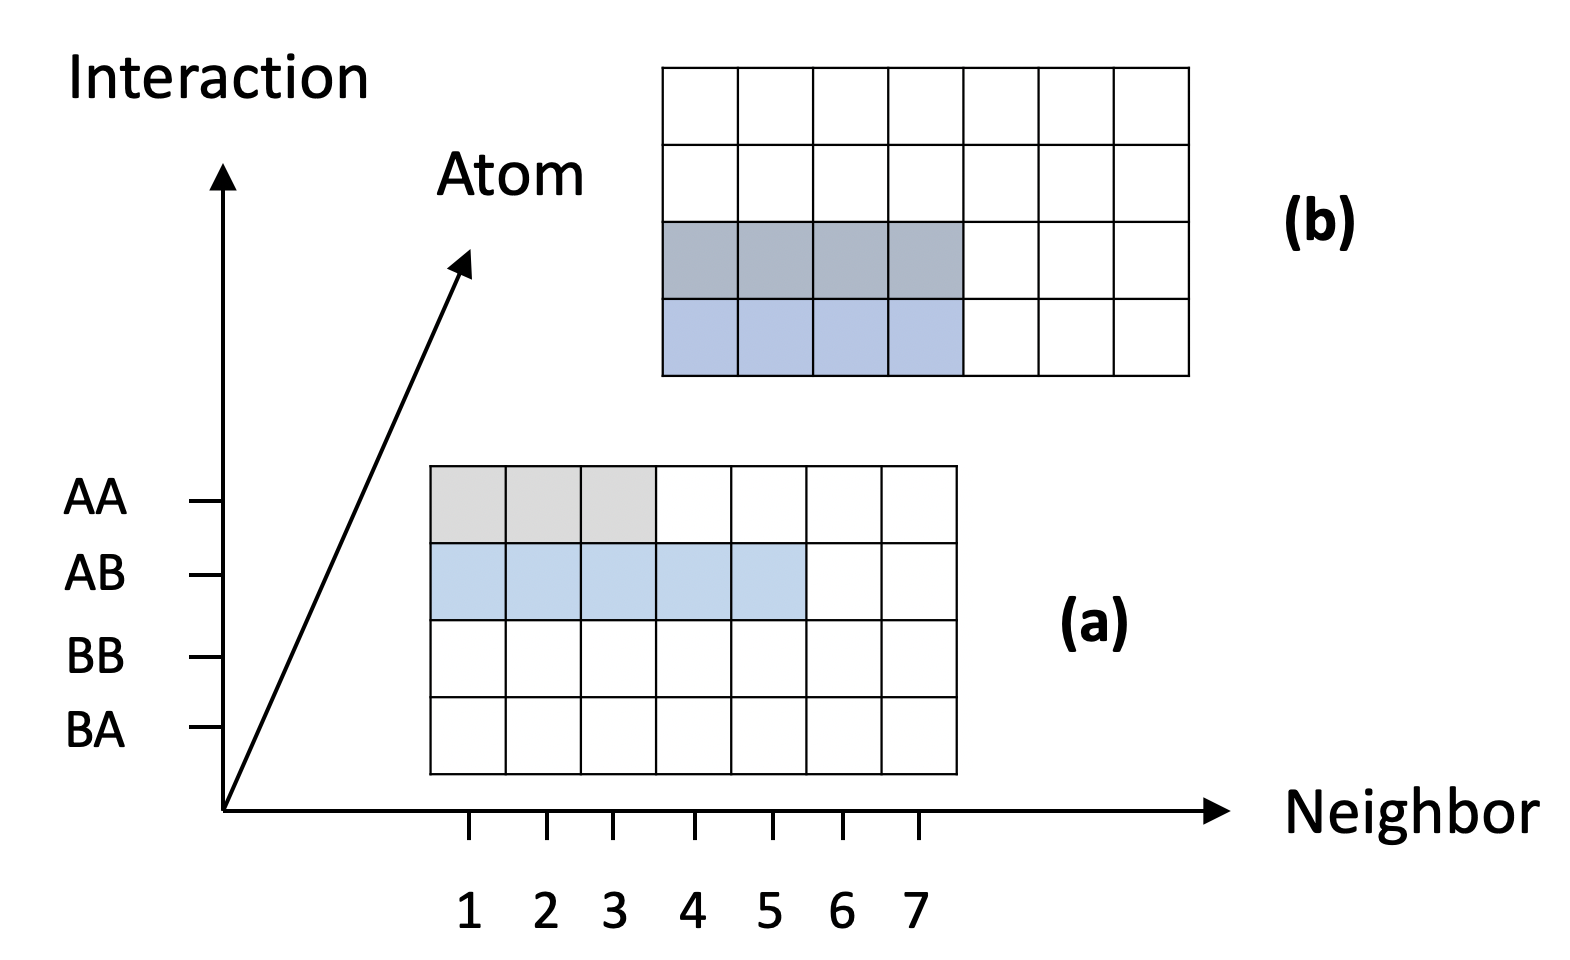
\includegraphics[scale=0.3]{figures/transformation.png}
\caption{\label{fig:transformation} Visualization of the descriptor matrix 
$\mathbf{G}'$ of the binary AB system and $\nnl$ is 7. Non-colored cells are 
padded zeros. \textbf{(a)} is a sample $\mathbf{g}_i$ of A-type atom and 
\textbf{(b)} represents a B-type atom.}
\end{figure}

Fig \ref{fig:transformation} is the visualization of the descriptor matrix 
$\mathbf{G}'$. $\mathbf{G}'$ has three axes: the neighbor axis, the interaction 
axis and the atom axis. $\nnl$ is the maximum of the neighbor axis (in this case 
$\nnl = 7$). For the binary AB system there are four types of interactions: AA, 
AB, BB and BA. \textbf{(a)} and \textbf{(b)} are samples of $\mathbf{g}_i$ for 
A-type atoms and B-type atoms.

% -----------
% Section 2.C Functions
% -----------
\subsection{Functions}
\label{sec:functions}

In this work, we use the EAM potential published by Zhou, Johnson and Wadley 
(Zjw04) \cite{ZJW0,ZJW1,ZJW2} as an example to validate our machine learning 
approach. Zjw04 is a quite popular EAM potential. In the Zjw04 potential, the 
electron density function has the following form:
\begin{equation}
\label{eq:zjw04_rho}
\rho_{b}(r) = \frac{
    f_{e} \exp\left[ -\beta\left( r/r_{e} - 1 \right) \right]
}{
    1 + \left(r/r_{e} - \lambda\right)^{20}
}
\end{equation}
where $r_e$ is a constant equal to equilibrium spacing between nearest neighors, 
$f_{e}$, $\beta$, $\lambda$ are adjustable parameters. The pairwise potential 
between the same species can be computed with:
\begin{equation}
\label{eq:zjw04_phi_aa}
\phi_{aa}(r) = 
\frac{A \exp\left[ -\alpha\left( r/r_{e} - 1 \right) \right]}
     {1 + \left(r / r_{e} - \kappa\right)^{20}} - 
\frac{B \exp\left[ -\beta\left( r/r_{e} - 1 \right) \right]}
     {1 + \left(r / r_{e} - \lambda\right)^{20}}
\end{equation}
where $A$, $B$, $\alpha$ and $\kappa$ are also trainable parameters, $\beta$ and 
$\kappa$ are used in Equation \ref{eq:zjw04_rho} already. For the pairwise 
interaction between two atoms of different species, the interpolation form is 
used:
\begin{equation}
\label{eq:zjw04_phi_ab}
\phi_{ab}(r) = \frac{1}{2}\left(
    \frac{\rho_{b}(r)}{\rho_{a}(r)}\phi_{aa}(r) +
    \frac{\rho_{a}(r)}{\rho_{b}(r)}\phi_{bb}(r) 
\right)
\end{equation}
The embedding function has a more complicated form as it requires to fit a much 
wider range of electron density values:
\begin{equation}
\label{eq:zjw04_embed}
F(\rho) = \begin{cases}
    \sum_{i=0}^{3}{F_{ni}\left( \frac{\rho}{\rho_n} - 1 \right)^{i}} &
    \rho < \rho_{n} \\
    \sum_{i=0}^{3}{F_{i}\left( \frac{\rho}{\rho_e} - 1 \right)^{i}} &
    \rho_{n} \leq \rho < \rho_{0} \\
    F_{e}\left[ 
        1 - \eta\ln\left( \frac{\rho}{\rho_s}\right) 
    \right](\frac{\rho}{\rho_s})^{\eta} & \rho_{0} \leq \rho
\end{cases}
\end{equation}
where $F_{ni}$, $F_{i}$, $\rho_e$, $\rho_s$, $\eta$ and $F_{e}$ are trainable 
parameters, $\rho_n=0.85\rho_e$ and $\rho_0=1.15\rho_e$. For each metal, there 
are 15 adjustable parameters. The original embedding potential is a stepwise 
function. Thus, the minimization requires some tricks to ensure its continuity.
To make it simpler, we slightly modified Equation \ref{eq:zjw04_embed}:
\begin{align}
\label{eq:zjw04xc_embed}
F(\rho) 
= & c_1 \cdot
\sum_{i=0}^{3}{F_{ni}\left( \frac{\rho}{\rho_n} - 1 \right)^{i}} \nonumber \\
+ & c_2 \cdot 
\sum_{i=0}^{3}{F_{i}\left( \frac{\rho}{\rho_e} - 1 \right)^{i}} \nonumber \\
+ & c_3 \cdot
F_{e}\left[1 - \eta\ln\left( \frac{\rho}{\rho_s}\right)\right]
(\frac{\rho}{\rho_s})^{\eta} \\
\label{eq:frho_c1}
c_{1} = & \frac{1}{1 + e^{-2\left(\rho_{n} - \rho\right)}} \\
\label{eq:frho_c3}
c_{3} = & \frac{1}{1 + e^{-2\left(\rho - \rho_{0}\right)}} \\
c_{2} = & 1 - c_1 - c_3
\end{align}
$c_1$ and $c_3$ are just damping factors calculated by the sigmoid 
functions (Equations \ref{eq:frho_c1} and \ref{eq:frho_c3}).

The dipole ($\mu_{ab}$) and quadrupole ($\lambda_{ab}$) functions have the same 
form (developed by Mishin \cite{ADP0}):
\begin{align}
\label{eq:adp_dipole}
\mu_{ab}(r) & = \left[
    d_{1}^{ab} \exp\left( -d_{2}^{ab}r \right) + d_{3}^{ab}
\right] \psi\left( \frac{r - r_{0}}{r_{h}} \right) \\
\omega_{ab}(r) & = \left[
    q_{1}^{ab} \exp\left( -q_{2}^{ab}r \right) + q_{3}^{ab}
\right] \psi\left( \frac{r - r_{0}}{r_{h}} \right)
\end{align}
where $d_{i}$, $q_{i}$, $r_0$ and $r_{h}$ are trainable parameters and $\psi(x)$
is a damping function:
\begin{equation}
\label{eq:mishin_cutoff}
\psi(x) = \begin{cases}
    0 & x \ge 0 \\
    \frac{x^4}{1 + x^4} & x < 0 
\end{cases}
\end{equation}

% -----------
% Section 2.D Physical constraints
% -----------
\subsection{Physical constraints}
\label{sec:constraints}

Physical constraints are quite common in fitting traditional empirical 
potentials. Physical constraints are typically static (cohesive energy, elastic 
constants, etc) collected from experiments and they can be very effective when 
training data is limited. For example, the cohesive energy, bulk modulus, 
vacancy formation energy and other constraints were used to develop the original 
Zjw04 potential. Mishin et al adopted the Rose universal equation of state to 
ensure the performaces of his ADP potentials in the high pressure region. 
However, such constraints are really rare in developing MILPs. One possible 
explanation may be these constraints are generally derived properties and 
implementing them in the loss function are technically difficult.

In this work, we successfully integrated two constraints into the total loss:
the Rose equation of state (EOS) \cite{Rose0,Rose1,Rose2} constraint and the 
elastic tensor constraint. These two losses will be discussed later. The details 
of their implementations will be described in another paper.

The Rose constraint incoporates the universal equation of state (Rose et al) 
into the total loss function. The Mishin-modified equation 
\begin{equation}
\label{eq:rose_eos}
E(x) = E_{0}\left[
    1 + \alpha x + \beta \alpha^3 x^3 \frac{2x + 3}{(x - 1)^2} \right]
    e^{-\alpha x}
\end{equation}
is used because the original form tends to underestimate energies under high 
pressures. In Equation \ref{eq:rose_eos}, $E_{0}$ is the energy of the 
equilibrium structure, $x = a / a_{0} - 1$ is the relative isotropic scaling 
factor ($a$ is the lattice constant), $\beta$ is a chosen parameter and 
\begin{equation}
\label{eq:rose_alpha}
\alpha = \sqrt{-\frac{9 V_{0} B }{E_{0}}}
\end{equation}
where $V_0$ is the equilibrium volume and $B$ is the corresponding bulk modulus. 
The adoption of the Rose constraint guarantees the exact predictions of bulk 
modulus and the energy-volume curve. The loss of the Rose EOS constraint 
$\mathbf{L}^{\mathrm{Rose}}$  is measured as the 2-norm of the energy 
differences between $E(x)^{\mathrm{dft}}$ and their corresponding predicted 
$E(x)$: 
\begin{equation}
\label{eq:rose_loss}
\mathbf{L}^{\mathrm{Rose}} = \sum_{\Omega}{
    \sqrt{\sum_{i}{\left(E(x_i) - E(x_i)^{\mathrm{dft}}\right)^2}}
}
\end{equation}
Here $\Omega$ denotes all selected crystals. In this work, for each included 
crystal, we use the same choices of $x$, which determines the fitting region: 
$x_{i} = x_{0} + \Delta x \cdot i, x_{0} = -0.1, N_{t}^{\mathrm{max}} = 20, 
\Delta x=0.01$. (-10\% to +10\% of the equilibrium volume). In this work, 
$\beta^{\mathrm{Ni}}$ is 0.005 and $\beta^{\mathrm{Mo}}$ is 0.008.
 
Elastic tensor is also a popular constraint for tuning empirical potentials but 
rarely used directly in optimizing MILPs. Shyue Ping Ong used this constraint in 
the outer loop (the global optimization based property-matching step) to find 
optimal parameters of SNAP potentials. 

In this work, we find a straightforward way to use elastic tensor directly as a 
constraint. Given an equilibrium crystal structure, its elastic constant 
$c_{ijkl}$ can be derived from $E^{total}$ directly \cite{Elastic}:
\begin{align}
\label{eq:virial}
V \cdot \epsilon & = -\mathbf{F}^{T}\mathbf{R} + \left(
    \frac{\partial E^{total}}{\partial \mathbf{h}}\right)^T \mathbf{h} \\ 
\label{eq:cijkl}
c_{ijkl} |_{\epsilon \to 0, \mathbf{F} \to 0} & = \frac{1}{V}\left[
    \left( 
        \frac{\partial{\epsilon_{ij}}}{\partial{\mathbf{h}}}
    \right)^{\mathrm{T}}\mathbf{h}
\right]_{kl}
\end{align}
where $V$ is the volume, $\epsilon$ is the $3 \times 3$ virial stress tensor, 
$\mathbf{h}$ is the \textit{row-major} $3 \times 3$ lattice tensor, $\mathbf{F}$ 
and $\mathbf{R}$ are $N \times 3$ matrices representing the total forces and 
atomic positions.

In this work, the loss $\mathbf{L}^{\mathrm{elastic}}$ contributed by the 
elastic tensor is also measured by the RMSE between $c_{ijkl}$ and 
$c_{ijkl}^{\mathrm{dft}}$:
\begin{align}
\label{eq:cijkl_loss}
\mathbf{L}^{\mathrm{elastic}} 
& = \sum_{\Omega}{\left(
    \omega_{\Omega} \cdot \mathbf{RMSE}_{\Omega} 
    + ||\epsilon|| + ||\mathbf{F}||
\right)}
 \\
\label{eq:cijkl_loss_gate}
\omega_{\Omega} & = \mathbf{ReLU}(\mathbf{MAE}_{\Omega} - \tau) \\
\label{eq:relu}
\mathbf{ReLU}(x) & = \begin{cases}
    x & x \ge 0 \\
    0 & x < 0
\end{cases}
\end{align}
where $\sum_{\Omega}$ loops through all included crystals, 
$\mathbf{MAE}_{\Omega}$ and $\mathbf{RMSE}_{\Omega}$ are the mean absolute error 
and root mean squared error between predicted elastic constants and DFT elastic 
constants. $\tau$ is a pre-selected gate parameter. 
When $\mathbf{MAE}$ is below $\tau$, $\mathbf{L}^{\mathrm{elastic}}$ will not 
contribute to the total loss. In this work, $\tau$ is set to 2 GPa.

The adoption of physical constraints in optimizing MLIPs can be very helpful. 
Without any physical constraint, adding high-quality data points is, perhaps, 
the only effective way to tune MLIPs for specific purposes. On the contrast, 
with physical constraints very few training samples are sufficient.
As an example, the elementary SNAP potentials (Mo, Ni) were fitted with just 
hundreds of structures but they performed quite well on elastic constants and 
surface energies, as in the outer loop \cite{SNAP_Mo} of the fitting process 
such material properties were already used. One must also note that data 
consistency is important. Physical constraints are just supplementary roles in 
developing MLIPs, so they are preferred to be measured with first-principle 
calculations.

% % % % % % % % % % % % % % % % % % % % % % % % % % % % % % % % % % % % % % % %
% 
% Figure: Ni - EAM - Plot
%
% % % % % % % % % % % % % % % % % % % % % % % % % % % % % % % % % % % % % % % %
\begin{figure*}
\centering
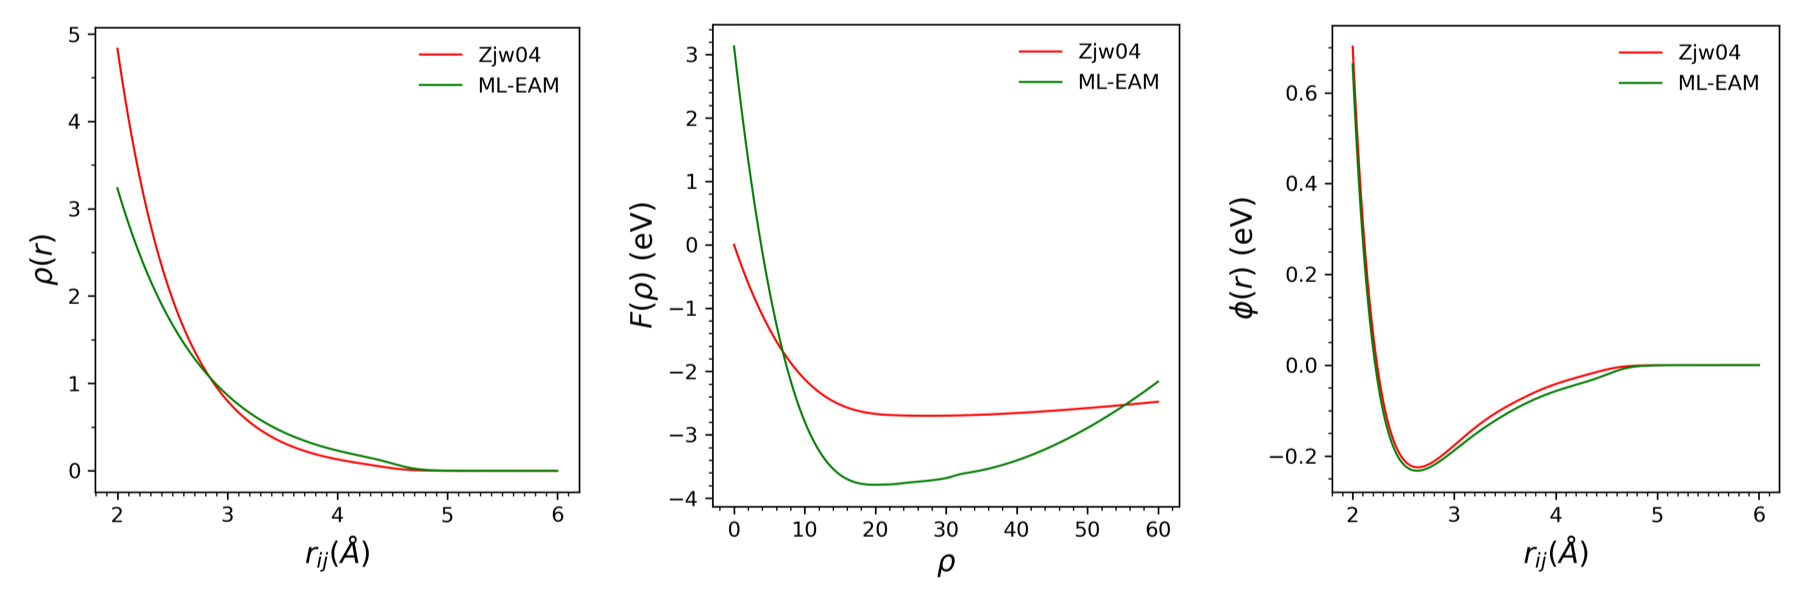
\includegraphics[scale=0.57]{figures/Ni_eam.png}
\caption{\label{fig:Ni_eam} $\rho(r)$, $F(\rho)$ and $\phi(r)$ of the original 
Zjw04 EAM and the machine learned EAM (ML-EAM).}
\end{figure*}

% % % % % % % % % % % % % % % % % % % % % % % % % % % % % % % % % % % % % % % %
% 
% Figure: Mo - EAM/ADP - Plot
%
% % % % % % % % % % % % % % % % % % % % % % % % % % % % % % % % % % % % % % % %
\begin{figure}[htp]
\centering
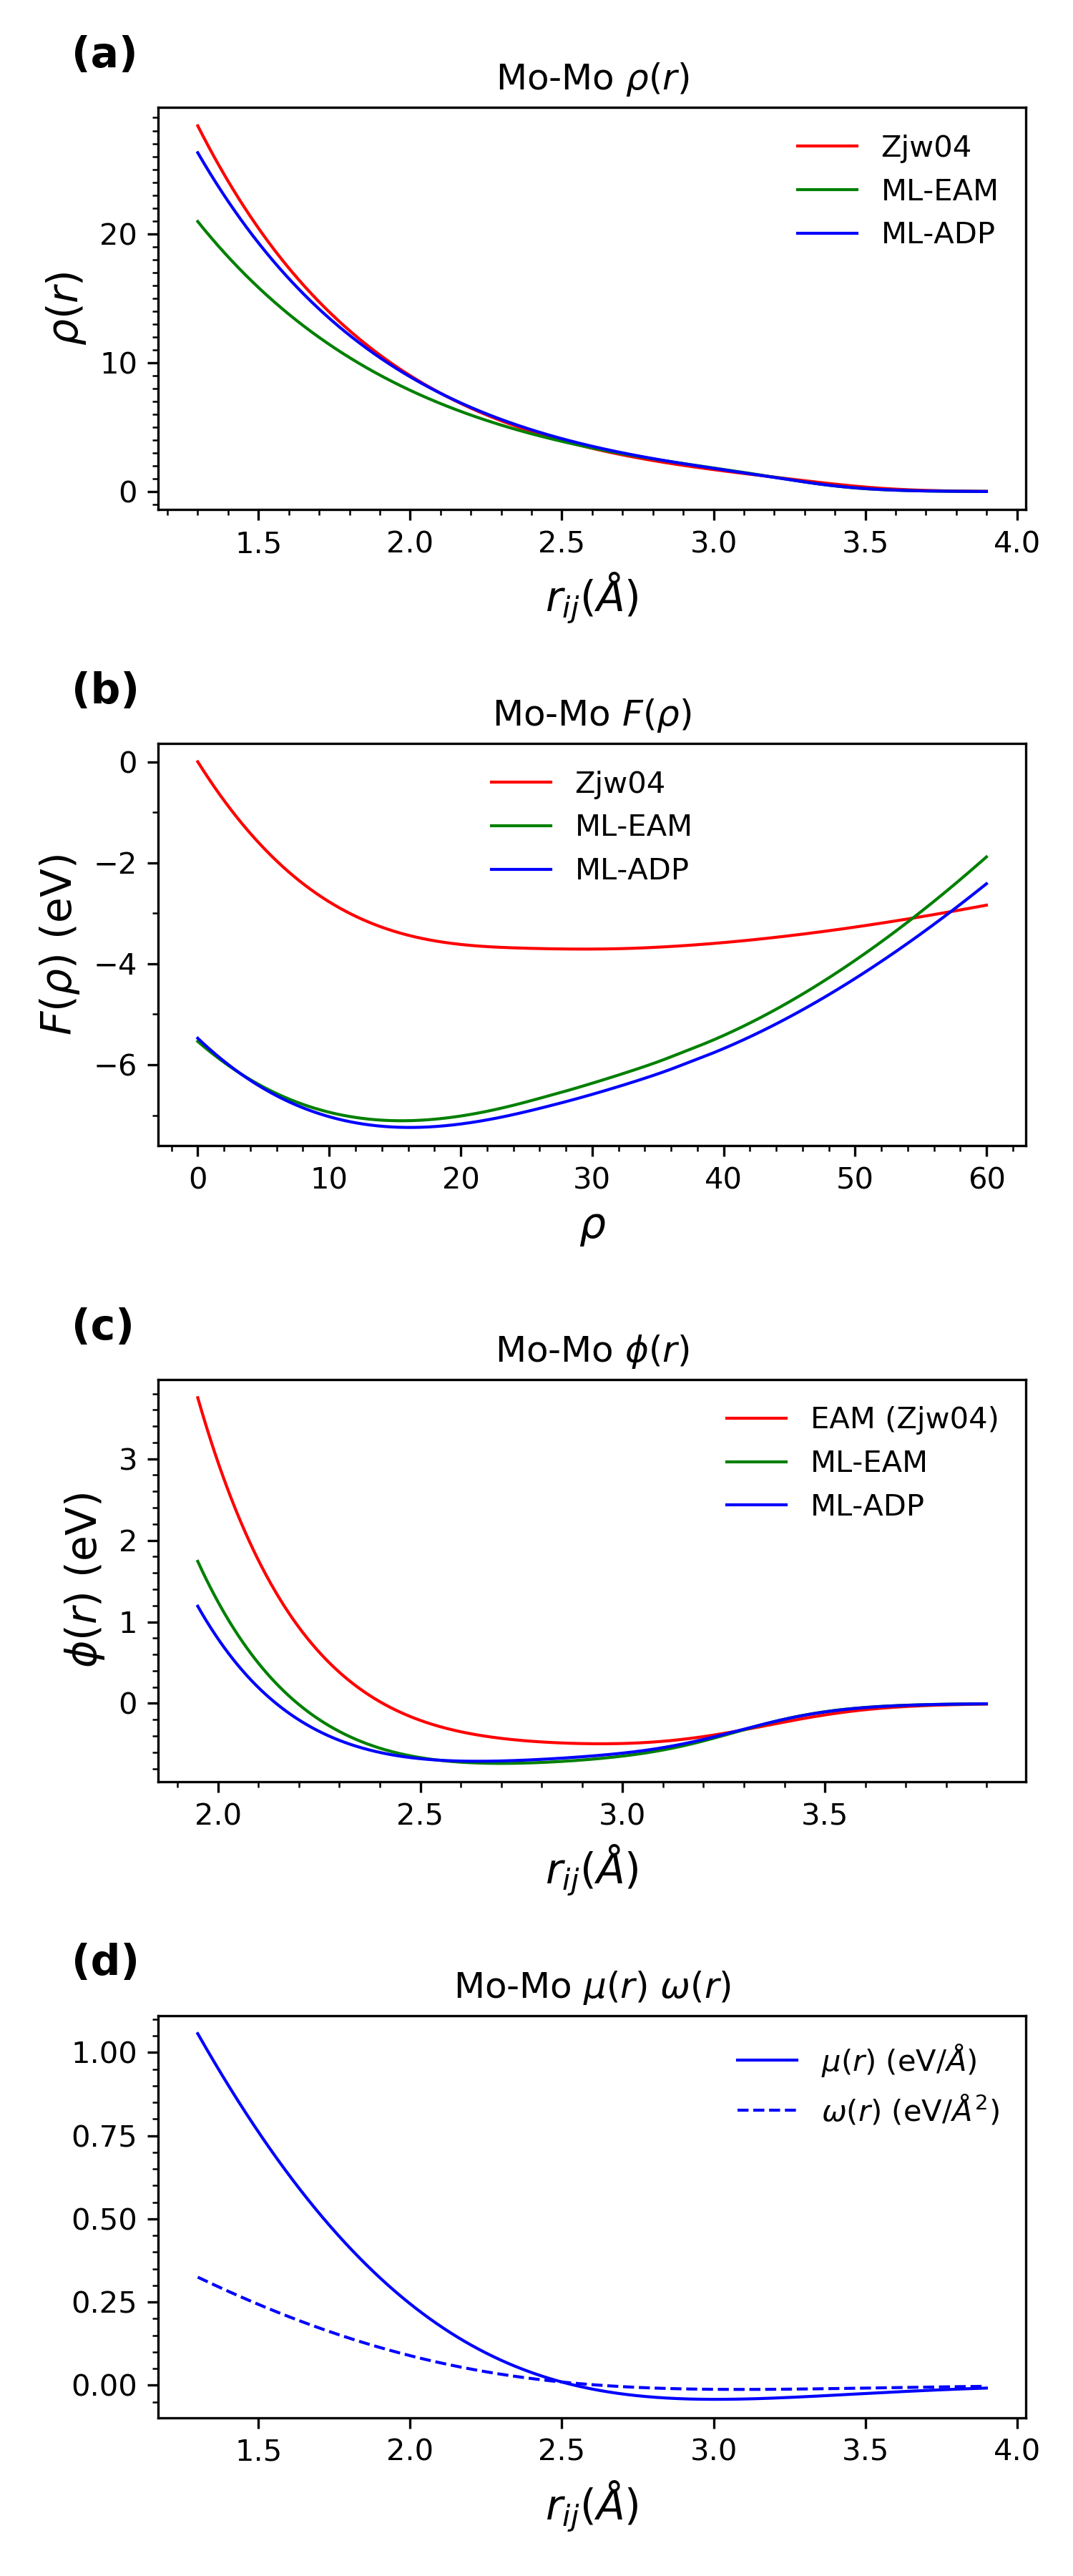
\includegraphics[scale=0.6]{figures/Mo_eam_adp.png}
\caption{\label{fig:Mo_eam_adp} $\rho(r)$, $F(\rho)$, $\phi(r)$ of the original 
Zjw04 EAM, ML-EAM and ML-ADP for elementary Mo. \textbf{(d)} shows the $\mu(r)$ 
and $\omega(r)$ of ML-ADP.}
\end{figure}

% % % % % % % % % % % % % % % % % % % % % % % % % % % % % % % % % % % % % % % %
% 
% Table: Ni / Mo MAEs
%
% % % % % % % % % % % % % % % % % % % % % % % % % % % % % % % % % % % % % % % %
\begin{table}
\centering
\begin{tabular}{lccccc}
\hline
            &    & EAM\cite{ZJW2} & SNAP\cite{SNAP} & ML-EAM & ML-ADP \\
\hline
Energy     & Ni & 10.6           & 1.2             & 3.9    &        \\
(meV/atom) & Mo & 58.9           & 13.2            & 23.8   & 18.7   \\
\hline
Force      & Ni & 0.06           & 0.05            & 0.05   &        \\
(eV/\AA)   & Mo & 0.31           & 0.25            & 0.30   & 0.29   \\
\hline
\end{tabular}
\caption{\label{table:Mo_Ni_mae} Comparisons of the energy and force MAEs of 
elementary Ni and Mo. 
}
\end{table}

% % % % % % % % % % % % % % % % % % % % % % % % % % % % % % % % % % % % % % % %
% 
% Table: Ni - Material Properties
%
% % % % % % % % % % % % % % % % % % % % % % % % % % % % % % % % % % % % % % % %
\begin{table*}
\centering
\begin{tabular}{lccccc}
\hline
                              & DFT  & SNAP \cite{SNAP} & EAM              & ML-EAM         & Exp.                           \\
\hline
$T_{m}$(K)                    &      & 1785             & 1520 \cite{ZJW2} & 1520           & 1728                           \\
$c_{11}$ (GPa)                & 276  & 276 (0.0\%)      & 248 (-10.1\%)    & 274 (-0.7\%)   & 261 \cite{Ni_Elastic_Exp}      \\
$c_{12}$ (GPa)                & 159  & 159 (0.0\%)      & 147 (-7.5\%)     & 163 (2.5\%)    & 151 \cite{Ni_Elastic_Exp}      \\
$c_{44}$ (GPa)                & 132  & 132 (0.0\%)      & 125 (-5.3\%)     & 131 (-0.8\%)   & 132 \cite{Ni_Elastic_Exp}      \\
$B_{\mathrm{VRH}}$ (GPa)      & 198  & 198 (0.0\%)      & 181 (-8.6\%)     & 195 (-1.5\%)    & 188                           \\
$G_{\mathrm{VRH}}$ (GPa)      & 95   & 95 (0.0\%)       & 87 (-8.4\%)      & 93 (-2.1\%)    & 93                             \\
$\mu$                         & 0.29 & 0.29 (0.0\%)     & 0.29 (0.0\%)     & 0.29 (0.0\%)   & 0.29                           \\
$E_{v}$ (eV)                  & 1.46 & 1.68 (15.1\%)    & 1.68 (15.1\%)    & 1.71 (17.1\%)  & 1.54–1.80 \cite{Ni_EvEmEa_Exp} \\
$E_{m}$ (eV)                  & 1.12 & 1.07 (-4.5\%)    & 0.90 (-19.6\%)   & 0.87 (-22.3\%) & 1.01–1.48 \cite{Ni_EvEmEa_Exp} \\
$E_{a} = E_{v} + E_{m} $ (eV) & 2.58 & 2.75 (6.6\%)     & 2.58 (0.0\%)     & 2.58 (0.0\%)   & 2.77–2.95 \cite{Ni_EvEmEa_Exp} \\
\hline
\end{tabular}
\caption{\label{table:Ni_properties} Comparison of the calculated and 
experimental material properties of elementary fcc Ni. $T_{m}$ is the melting 
point. $c_{ij}$ represents elastic constants. $E_{v}$ and $E_{m}$ are vacancy 
formation energy and migration energy, respectively. SNAP refers to the 
elementary Ni SNAP model.
}
\end{table*}

% -----------
% Section 2.E Implementation
% -----------
\subsection{Implementation}
\label{sec:implementation}

The implementation of the machine learned EAM and the physical
constraints are beyond the scope of this work. The details will be discussed
in another paper. Here, we will give a brief description.

Both ML-EAM and ML-ADP are implemented within Google's TensorFlow. The 
virtual-atom approach (VAP) is adopted \cite{TensorAlloy} so that we can 
construct a computation graph from atomic positions to total energy directly. 
Thus, atomic forces (Equation \ref{eq:forces}) and virial stress 
(Equation \ref{eq:virial}) can be derived by the AutoGrad module of TensorFlow 
automatically and efficiently. 
\begin{equation}
\label{eq:forces}
\mathbf{F} = -\frac{\partial E^{total}}{\partial \mathbf{R}}
\end{equation}
This direct computation graph also plays a key role in computing analytical 
elastic tensor (Equation \ref{eq:cijkl}) and the Rose loss 
(Equation \ref{eq:rose_eos}).
 
To find optimal parameters of the funcitons in section \ref{sec:functions}, the 
overall loss function shall be defined. Just like other machine learning tasks, 
the mini-batch stochastic gradient descent algorithm is used to minimize the 
loss function. Equation \ref{eq:loss} demonstrates the loss function used in 
this work:
\begin{align}
\label{eq:loss}
\mathbf{Loss} & = \sqrt{\frac{1}{N_{b}}\sum_{i=1}^{N_{b}}{\left(
    E_{i} - E_{i}^{\mathrm{dft}}
\right)^2}} \nonumber \\
& + \chi_{\mathrm{f}}\sqrt{
    \frac{1}{3\sum_{i}^{N_{b}}{N_i}}\sum_{i}^{N_b}{\sum_{j}^{N_i}{
        \sum_{\alpha}{
            \left(f_{ij\alpha} - f_{ij\alpha}^{\mathrm{dft}}\right)^2
        }
    }}
} \nonumber \\
& + \chi_{\mathrm{rose}}\mathbf{L}^{\mathrm{Rose}} 
+ \chi_{\mathrm{elastic}}\mathbf{L}^{\mathrm{elastic}}
\end{align} 
where $N_{b}$ is the batch size and $N_i$ is the number of atoms in structure 
$i$. $\chi_{\mathrm{f}}$, $\chi_{\mathrm{rose}}$ and $\chi_{\mathrm{elastic}}$ 
are overall weights of force, rose EOS and elastic contributions. 
The Adam optimizer \cite{adam} is used to minimize Equation \ref{eq:loss}. 
In most cases, we use 0.01 as the initial learning rate and the batch size 
ranges from 20 to 50. Since there are very few adjustable parameters compared 
with neural networks, the optimization typically needs very few epochs to 
converge. When the optimization is finished, the corresponding Lammps setfl 
potential file will be exported.

% % % % % % % % % % % % % % % % % % % % % % % % % % % % % % % % % % % % % % % %
% 
% Section 3. Results
%
% % % % % % % % % % % % % % % % % % % % % % % % % % % % % % % % % % % % % % % %
\section{Results}
\label{sec:results}

The public Ni-Mo dataset \cite{SNAP} is used to evaluate our approach. This 
dataset is provided by Shyue Ping Ong and co-workers along with their SNAP 
models. It contains 3973 different Ni-Mo solids. All calculations were done by 
VASP \cite{VASP} with the PBE \cite{PBE} functional and the projector 
augmented-wave approach \cite{PAW}. 

The optimized parameters are listed in the appendix.

% % % % % % % % % % % % % % % % % % % % % % % % % % % % % % % % % % % % % % % %
% 
% Section 3.A
%
% % % % % % % % % % % % % % % % % % % % % % % % % % % % % % % % % % % % % % % %
\subsection{Elementary Ni and Mo}
\label{sec:elementary}

% % % % % % % % % % % % % % % % % % % % % % % % % % % % % % % % % % % % % % % %
% 
% Figure: Surface Energy - Plot
%
% % % % % % % % % % % % % % % % % % % % % % % % % % % % % % % % % % % % % % % %
\begin{figure}
\centering
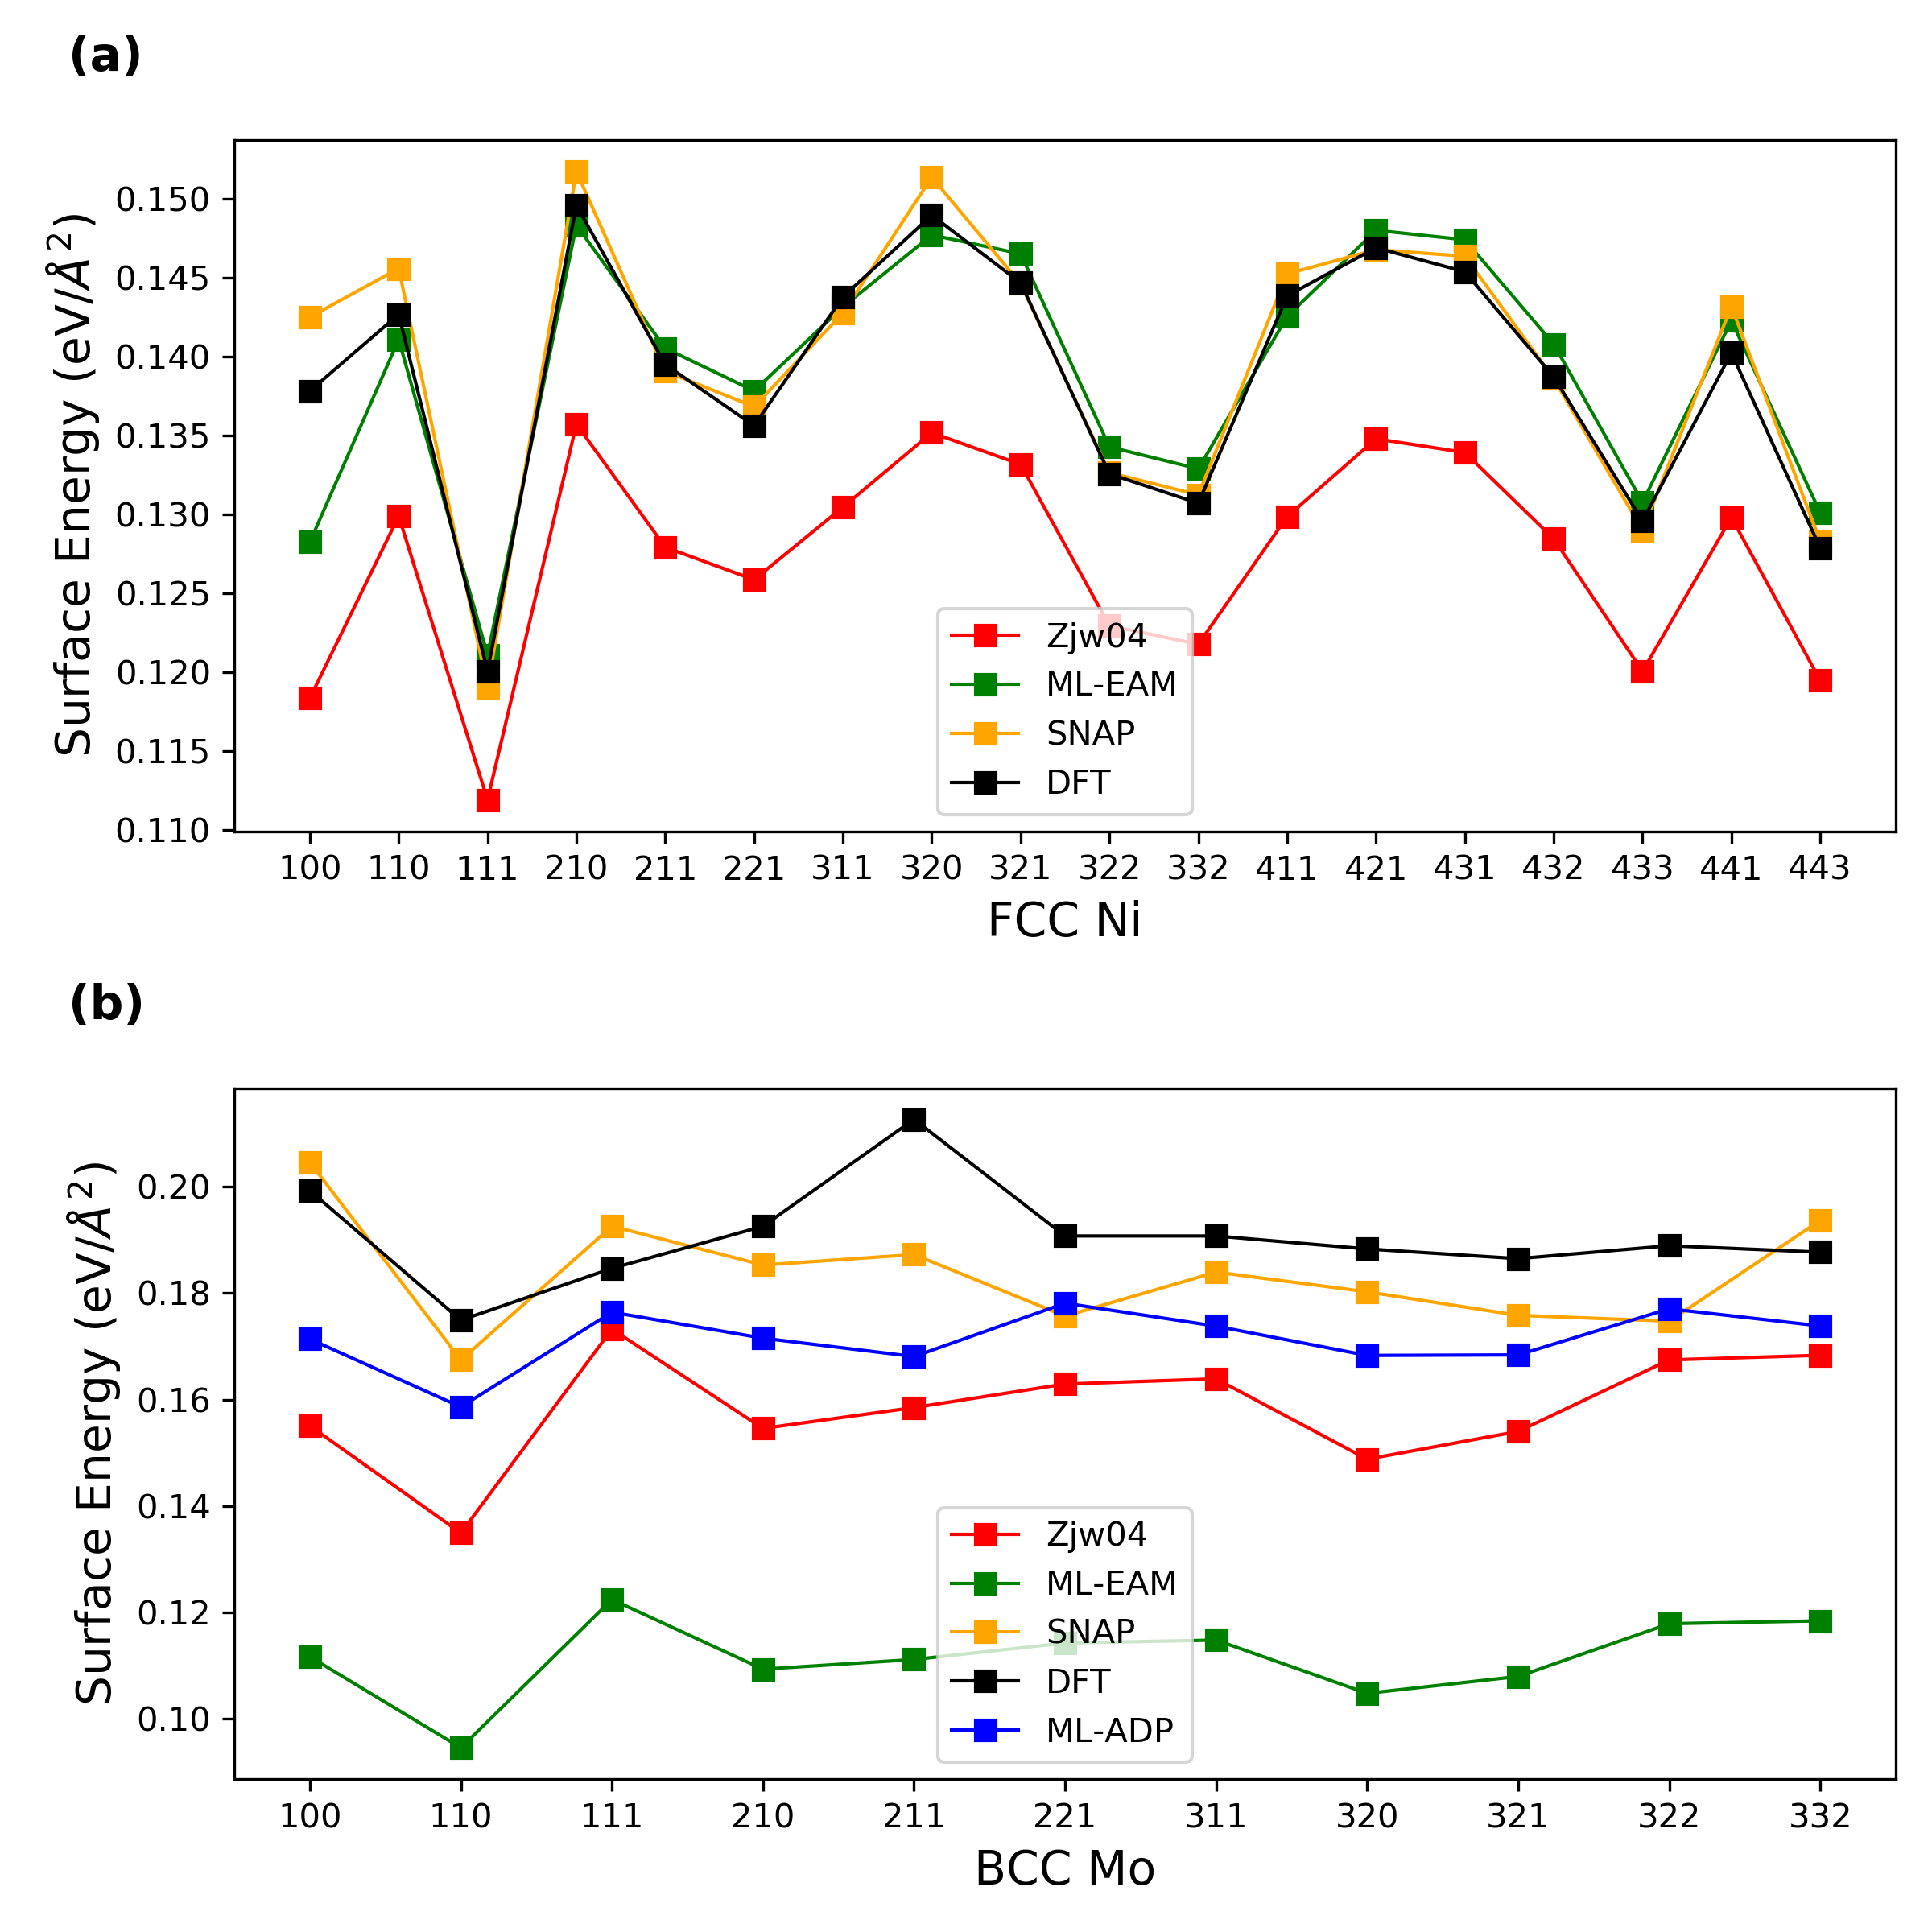
\includegraphics[scale=0.4]{figures/surface_energy.png}
\caption{\label{fig:surface_energy} Comparison of calculated surface energies of 
\textbf{(a)} fcc Ni and \textbf{(b)} bcc Mo.}
\end{figure}

We firstly use the two elementary datasets (Ni and Mo) to show our approach. These 
two datasets has 461 and 284 structures, respectively. 61 and 34 structures were 
randomly selected to form the test subsets. In these two experiments, 
$\chi_{\mathrm{f}}$, $\chi_{\mathrm{rose}}$ and $\chi_{\mathrm{elastic}}$ were 
set to 1, 3 and 0.05 respectively. The batch size was fixed to 25.

The original Zjw04 potentials were fitted to experimentally obtained quantities.
Thus, we use the relative MAE:
\begin{equation}
\mathbf{rMAE} = \frac{1}{N}\sum_{i=1}^{N}{
    | \frac{(E_i - E_i^{dft})}{N_i} - (E_{eq} - E_{eq}^{dft}) |
}
\end{equation}
to measure their performaces. Here $N_i$ is the number of atoms in structure 
$i$, $E_i$ is the Zjw04 energy of structure $i$ while $E_i^{dft}$ represents its 
corresponding DFT energy, $E_{eq}$ and $E_{eq}^{dft}$ refers to the equilibrium 
energy of Zjw04 and DFT, respectively.

Figure \ref{fig:Ni_eam} compares the $\rho(r)$, $F(\rho)$, $\phi(r)$, 
$\mu(r)$ and $\omega(r)$ functions. The differences between ML-EAM and ML-ADP 
$\rho(r)$, $\phi(r)$ and $F(\rho)$ are quite small. 

% % % % % % % % % % % % % % % % % % % % % % % % % % % % % % % % % % % % % % % %
% 
% Figure: Ni - EOS
%
% % % % % % % % % % % % % % % % % % % % % % % % % % % % % % % % % % % % % % % %
\begin{figure}
\centering
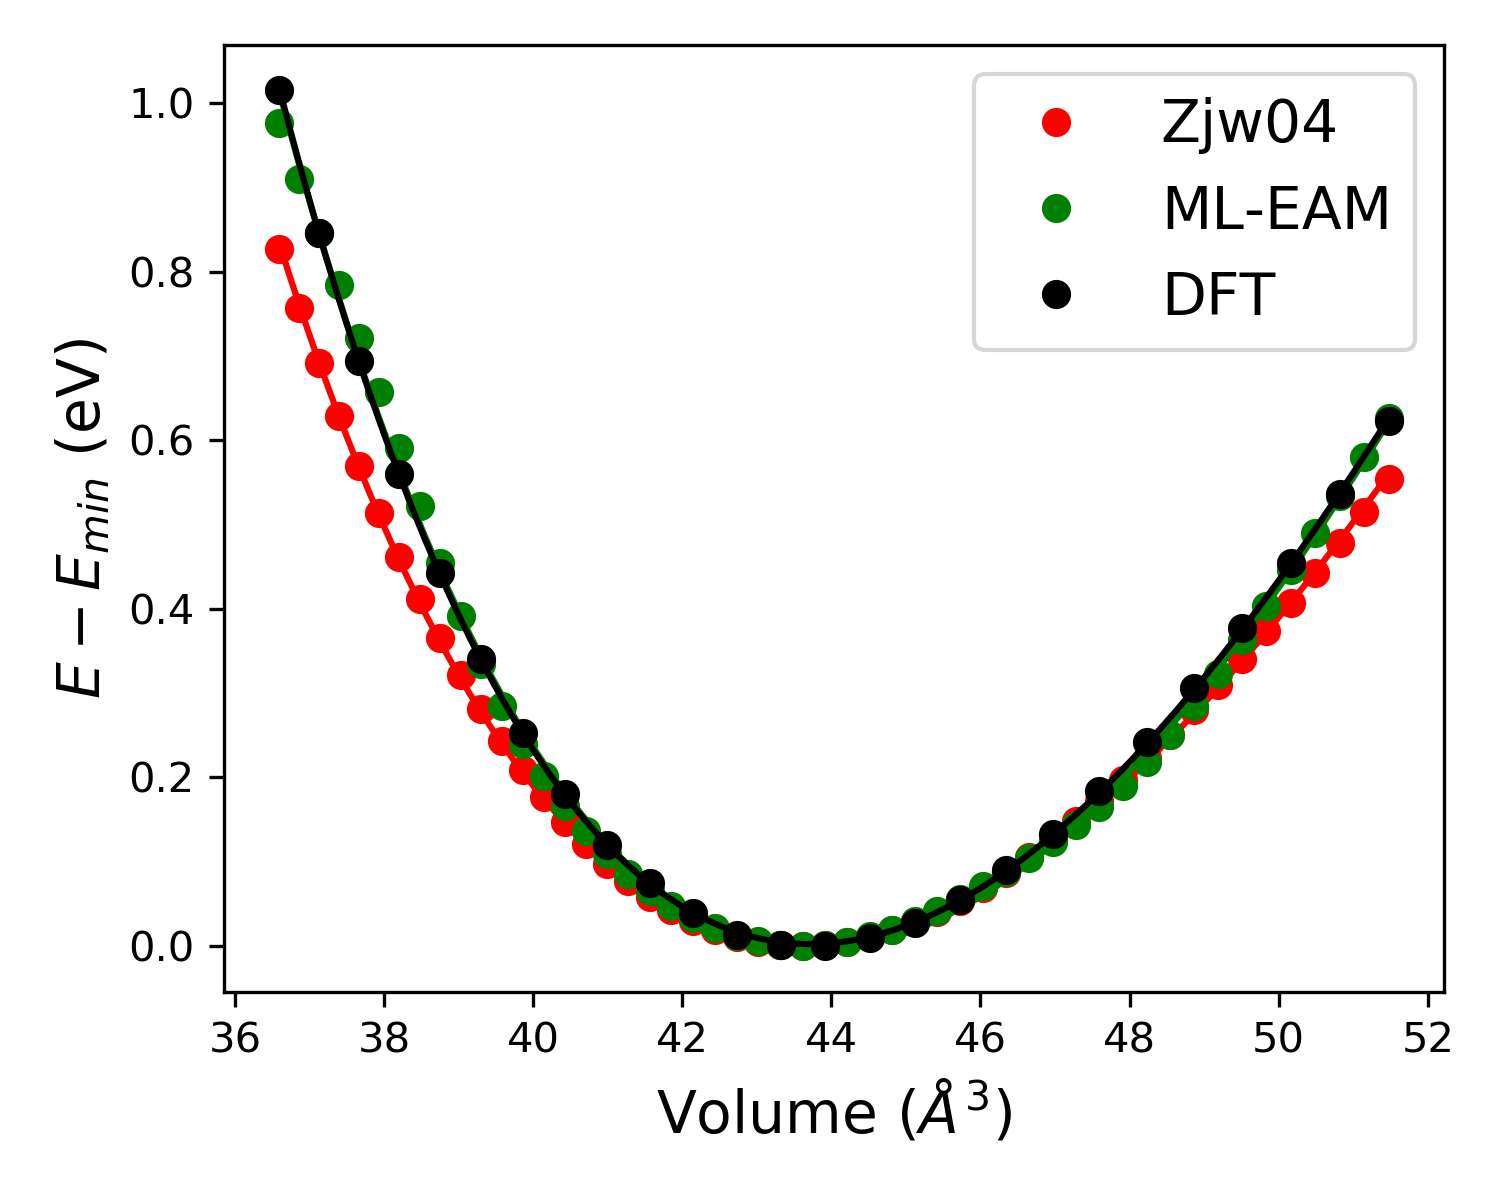
\includegraphics[scale=0.65]{figures/Ni_all_eos.png}
\caption{\label{fig:Ni_eos} The energy-volume curves of the original EAM, 
ML-EAM and DFT for the fcc Ni.}
\end{figure}

% % % % % % % % % % % % % % % % % % % % % % % % % % % % % % % % % % % % % % % %
% 
% Figure: Mo - EOS
%
% % % % % % % % % % % % % % % % % % % % % % % % % % % % % % % % % % % % % % % %
\begin{figure}
\centering
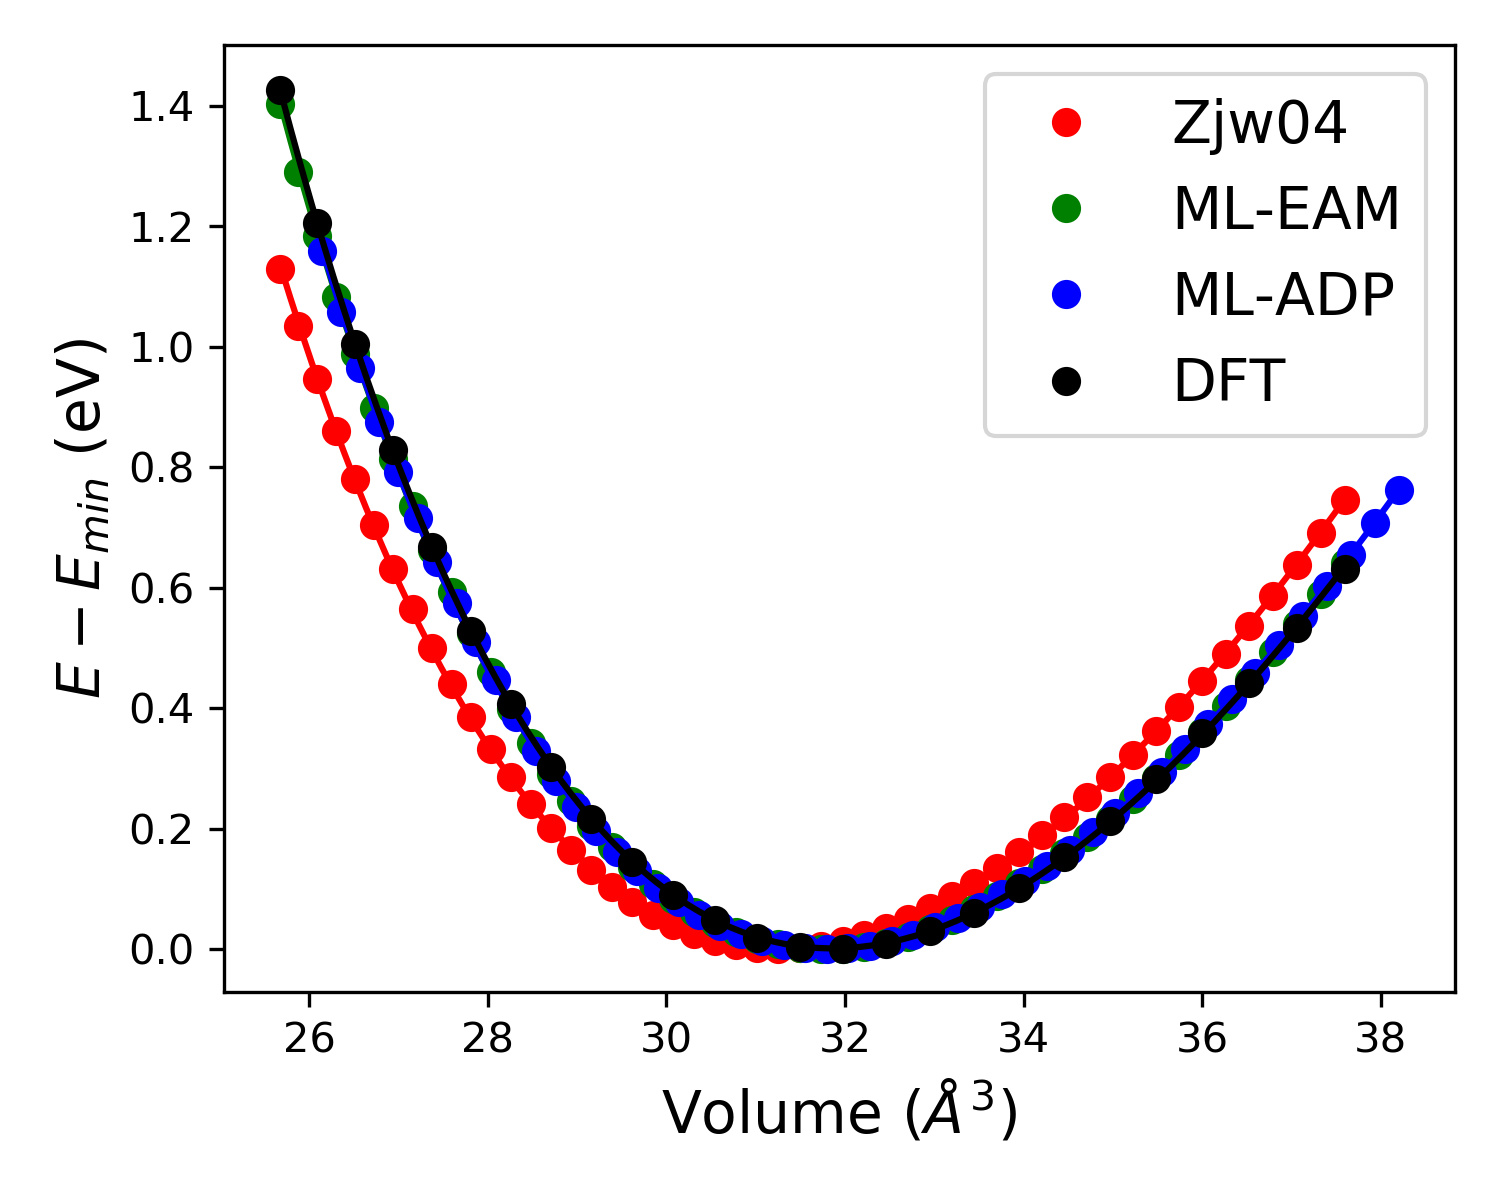
\includegraphics[scale=0.65]{figures/Mo_all_eos.png}
\caption{\label{fig:Mo_eos} The energy-volume curves of the original EAM, 
ML-EAM, ML-ADP and DFT for the bcc Mo.}
\end{figure}

For the Ni dataset, the original Zjw04 already has a reasonable performace. 
The energy \textbf{rMAE} is 10.6 meV/atom and the force MAE is just 0.06 eV/\AA 
on the entire dataset. Our machine learning approach can further enhance the 
performace. ML-EAM achieves 4.1 meV/atom and 0.05 eV/\AA on the test set and 
3.9 meV/atom and 0.05 eV/\AA on the entire dataset. ML-EAM is nearly as accurate 
as SNAP (1.2 meV/atom, 0.05 eV/\AA), but later has almost three orders of 
magnitude more computational expense. Figure \ref{fig:Ni_eam} demonstrates the 
$\rho(r)$, $F(\rho)$ and $\phi(r)$ functions before (Zjw04) and after machine 
learning optimization. The pairwise potential $\phi(r)$ almost remains the same 
while the embedding function $F(\rho)$ and the electron density function 
$\rho(r)$ changes significantly. Both $\rho(r)$ and $\phi(r)$ converge to zero 
at around $r=4.8$ \AA, which is rougly 2 times of the equilibrium spacing 
between nearest neighbors.

For the Mo dataset, the situation is quite different. The original Zjw04 has 
extremely large MAEs: the energy \textbf{rMAE} is $\sim 59$ meV/atom and the 
force MAE is more than 0.31 eV/\AA. Our method can significantly reduce the 
error: ML-EAM can achieve test MAEs of 23.8 meV/atom and 0.26 eV/\AA and overall
MAEs of 26.7 meV/atom and 0.30 eV/\AA. We also optimized an ADP potential for 
this dataset. Interestingly, ML-ADP gets better results: 20.6 meV/atom and 
0.24 eV\AA on the test set and 18.7 meV/atom and 0.29 eV/\AA on the entire 
dataset. On the contrast, the SNAP method (13.2 meV/atom, 0.25 eV/\AA) behaves 
slightly better than ML-ADP. But considering the computational cost, the 
performace of ML-ADP is totally acceptable. Figure \ref{fig:Mo_eam_adp} 
demonstrates the potential functions. The $\rho(r)$, $F(\rho)$ and $\phi(r)$ 
functions of ML-EAM and ML-ADP are quite similar. The additional accuracy of 
ML-ADP mainly comes from the dipole function $\mu(r)$. 

% % % % % % % % % % % % % % % % % % % % % % % % % % % % % % % % % % % % % % % %
% 
% Table: Mo - Material Properties
%
% % % % % % % % % % % % % % % % % % % % % % % % % % % % % % % % % % % % % % % %
\begin{table*}
\centering
\begin{tabular}{lcccccc}
\hline
                              & DFT  & SNAP \cite{SNAP_Mo} & EAM \cite{ZJW2} & ML-EAM         & ML-ADP         & Exp.                      \\
\hline
$T_{m}$(K)                    &      & 3000                & 3750            & 2840           & 2910           & 2890                      \\
$c_{11}$ (GPa)                & 472  & 473 (0.2\%)         & 457 (-3.2\%)    & 463 (-1.9\%)   & 469 (-0.6\%)   & 479 \cite{Mo_Elastic_Exp} \\
$c_{12}$ (GPa)                & 158  & 152 (-3.8\%)        & 168 (6.3\%)     & 153 (-3.2\%)   & 159 (0.6\%)    & 165 \cite{Mo_Elastic_Exp} \\
$c_{44}$ (GPa)                & 106  & 107 (0.9\%)         & 116 (9.4\%)     & 98 (-7.5\%)    & 102 (-3.8\%)   & 108 \cite{Mo_Elastic_Exp} \\
$B_{\mathrm{VRH}}$ (GPa)      & 263  & 259 (-1.5\%)        & 264 (0.4\%)     & 256 (-2.7\%)   & 262 (-0.4\%)   & 270 \cite{Mo_Elastic_Exp} \\
$G_{\mathrm{VRH}}$ (GPa)      & 124  & 126 (1.6\%)         & 127 (2.4\%)     & 118 (-4.8\%)   & 121 (-2.4\%)   & 125 \cite{Mo_Elastic_Exp} \\
$\mu$                         & 0.30 & 0.29 (-3.3\%)       & 0.29 (-3.3\%)   & 0.30 (0.0\%)   & 0.30 (0.0\%)   & 0.30                      \\
$E_{v}$ (eV)                  & 2.87 & 2.61 (-9.1\%)       & 3.02 (5.2\%)    & 1.96 (-31.7\%) & 2.51 (-12.5\%) &                           \\
$E_{m}$ (eV)                  & 1.12 & 1.39 (24.1\%)       & 1.54 (37.5\%)   & 1.33 (18.7\%)  & 1.06 (-5.3\%)  &                           \\
$E_{a} = E_{v} + E_{m} $ (eV) & 3.99 & 4.00 (-0.1\%)       & 4.56 (14.3\%)   & 3.29 (-17.5\%) & 3.57 (-10.5\%) & 4.00 \cite{Mo_Ea_Exp}     \\
\hline
\end{tabular}
\caption{\label{table:Mo_properties} Comparison of the calculated and 
experimental material properties of elementary bcc Mo. SNAP refers to the 
elementary SNAP Mo model.
}
\end{table*}

% % % % % % % % % % % % % % % % % % % % % % % % % % % % % % % % % % % % % % % %
% 
% Figure: Alloy EOS - Plot
%
% % % % % % % % % % % % % % % % % % % % % % % % % % % % % % % % % % % % % % % %
\begin{figure*}
\centering
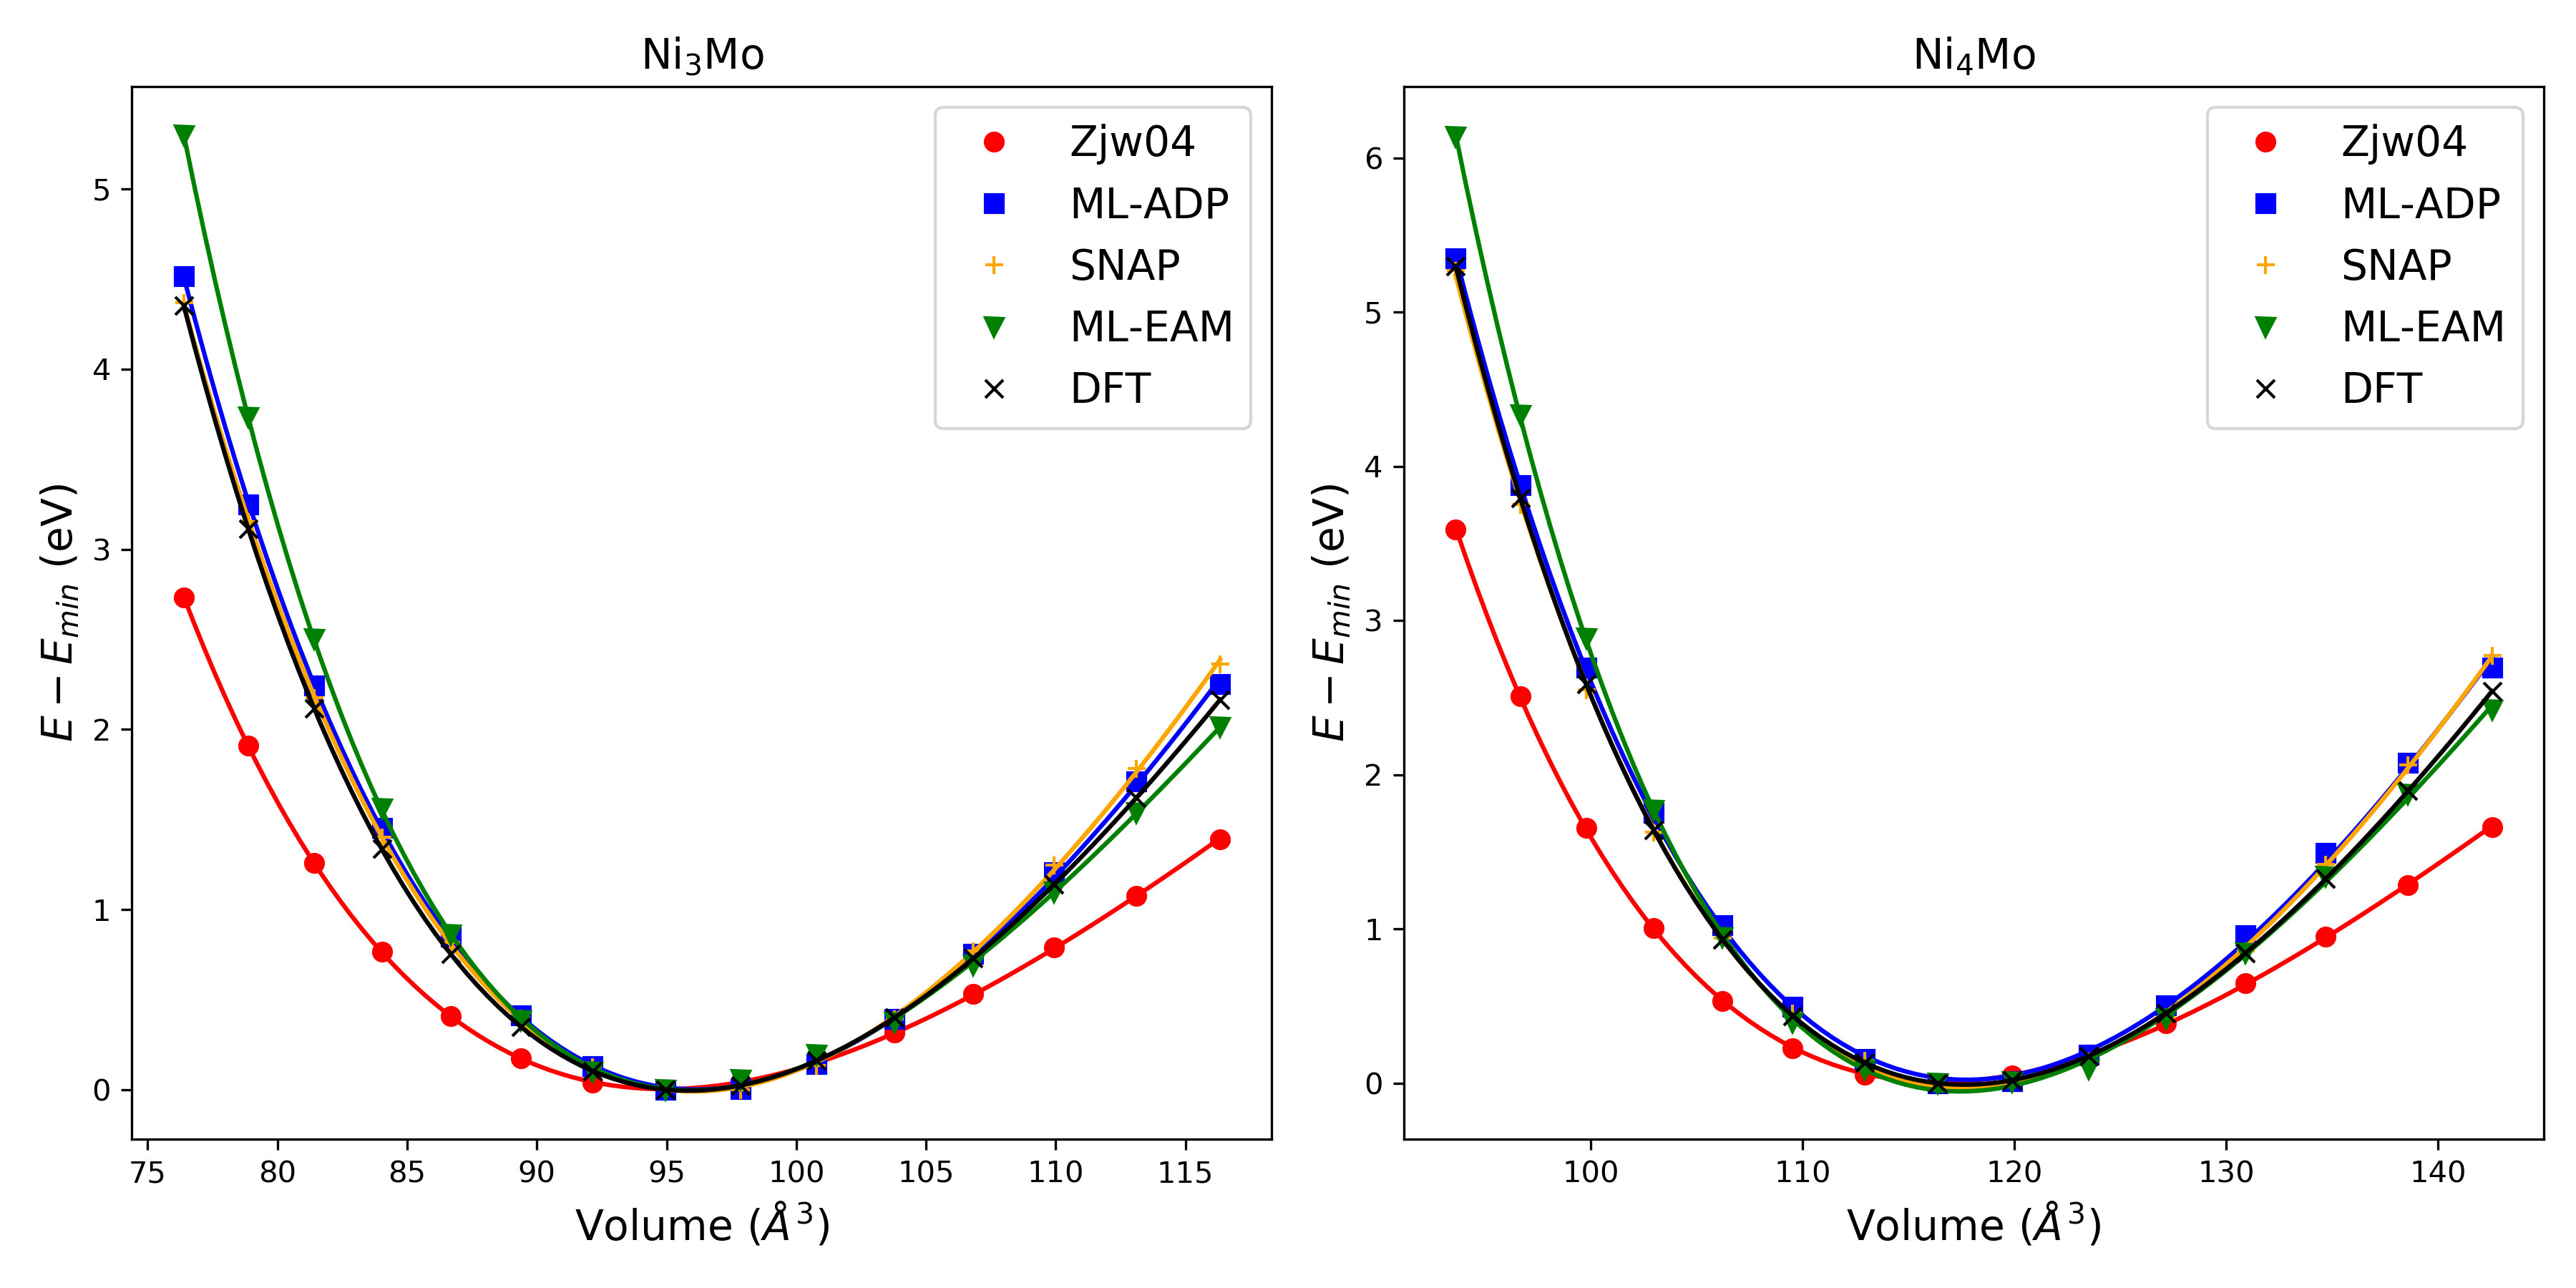
\includegraphics[scale=0.5]{figures/alloy_eos.png}
\caption{\label{fig:alloy_eos} Energy-volume curves of Ni$_3$Mo and Ni$_4$Mo 
obtained with the original Zjw04 EAM, ML-EAM, ML-ADP, SNAP and DFT.}
\end{figure*}

Figure \ref{fig:Ni_eos} and \ref{fig:Mo_eos} plot the equation of state 
curves. The fitting region ranges from 84\% to 118\% of the corresponding 
equilibrium volume. For both crystals, the original EAM significantly 
underestimate the energy at both tensile and compress strains. However, our 
constrained machine learning approach can fix this problem. The 
energy-volume curves of ML-EAM and ML-ADP overalp with the DFT curves very well. 

Table \ref{table:Ni_properties} and \ref{table:Mo_properties} summerize the 
predicted material properties of fcc Ni and bcc Mo, including the melting point 
$T_{m}$, the elastic constants ($c_{11}$, $c_{12}$ and $c_{44}$), the vacancy 
formation energy $E_{v}$, the migration energy $E_{m}$ and the activation energy 
$E_{a}$. The original Zjw04 potentials were developed by fitting material 
properties so they already perform well on these metrics. For the fcc Ni, the 
machine-learned EAM has gained better performances on predicting elastic 
constants. For the bcc Mo, ML-ADP not only gives quality predictions on elastic 
properties but also significantly reduces the error of predicting $E_m$. We also 
tested these models with surface energy, as shown in Fig 
\ref{fig:surface_energy}. One must note that all the slab structures are relaxed 
independently with corresponding potentials. For the fcc Ni, ML-EAM can give 
almost exactly the same results with DFT. For the more complicated bcc Mo, the 
central-force ML-EAM model becomes not that good due to the lacking of 
directional d bonding \cite{ADP0}. The angular correction, introduced by Mishin, 
shows its importance. ML-ADP can give comparable results to the SNAP method.

We further examined our ML-EAM and ML-ADP by calculating the melting temperature
of fcc Ni and bcc Mo using the solid-liquid coexistence approach. For fcc Ni, 
$30 \times 10 \times 10$ supercells were used and for bcc the supercells 
$30 \times 15 \times 15$ were used. The time step was set to 1 fs. The 
simulation for each temperature was carried out for at least 300 ps. 
For fcc Ni, $T_{m}$ remains the 
same for ML-EAM, 200 K lower than the experiment $T_m$. However, the calculated 
$T_{m}$ of Mo is greatly improved. The original Zjw04 $T_{m}$ is around 3750 K, 
800 K higher than experiment (2890 K) while both ML-EAM and ML-ADP can give 
quite accurate melting temperature. 

% % % % % % % % % % % % % % % % % % % % % % % % % % % % % % % % % % % % % % % %
% 
% Section 3.C
%
% % % % % % % % % % % % % % % % % % % % % % % % % % % % % % % % % % % % % % % %
\subsection{Mo-Ni}
\label{sec:alloy}

Secondly, we tested our method on the entire binary Mo-Ni dataset. 300 
structures were randomly chosen to be the test dataset and the rest 3673 
were used to train the potentials. $\chi_{\mathrm{f}}$, $\chi_{\mathrm{rose}}$ 
and $\chi_{\mathrm{elastic}}$ were set to 1, 1 and 0.05 respectively. The batch 
size was increased to 50. Only the equilibrium fcc Ni and bcc Mo are included in 
$\Omega$ of Equation \ref{eq:cijkl_loss} and \ref{eq:rose_loss}.

The original EAM uses a simplified combined form to describe the pairwise 
interaction of A-B (Equation \ref{eq:zjw04_phi_ab}). However, we did a minor 
modification: by adding more fitting parameters we use Equation 
\ref{eq:zjw04_phi_aa} directly. Thus, in total, there are 44 learnable 
parameters for ML-EAM and 68 for ML-ADP. One should note that in this section, 
SNAP, ML-EAM and ML-ADP all refer to their corresponding binary form.

Table \ref{table:MAE} summarizes the energy and force MAEs of SNAP, ML-EAM and 
ML-ADP on the different subsets. ML-ADP becomes the overally best. 
Both the energy MAE (19.6 meV/atom) and the force MAE (0.20 eV/\AA) are smaller 
than those of the binary SNAP (22.5 meV/atom and 0.23 eV/\AA). 
The pure Mo is still a challenge for ML-ADP as the energy and force MAEs are 
noticeably large but still much smaller than the original Zjw04 EAM. The binary 
SNAP predicts well on pure Ni and Mo. But ML-ADP outperforms the SNAP model on 
binary phases (Ni$_3$Mo, Ni-doped Mo and especially the Mo-doped Ni).
On the contrast, ML-EAM still performs significantly worse compared with ML-ADP 
due to the restriction of the central-force model, as discussed before. 
Interestingly, our results suggest that Mo-Ni dipole and quadrupole 
contributions are completely negligible (Figure S1 in the appendix). The Ni-Ni 
dipole and quadrupole interactions are an order of magnitude weaken than those 
of Mo-Mo. 

Figure \ref{fig:alloy_eos} demonstrates the energy-volume curves of Ni$_3$Mo and
Ni$_4$Mo. The original Zjw04 EAM can not properly describe the energy-volume 
relations of these two crystals in wide range. The ML-ADP curves agrees 
perfectly with the DFT curves. ML-EAM agrees well under tensile strains but 
overestimates the energy under compress strains. 

% % % % % % % % % % % % % % % % % % % % % % % % % % % % % % % % % % % % % % % %
% 
% Table: Mo-Ni MAE
%
% % % % % % % % % % % % % % % % % % % % % % % % % % % % % % % % % % % % % % % %
\begin{table*}
\centering
\begin{tabular}{lcccccccc}
\hline
                  & Model            & Mo   & Ni$_4$Mo & Ni$_3$Mo & Mo$_{\mathrm{Ni}}$ & Ni$_{\mathrm{Mo}}$ & Ni   & Overall \\
\hline
Energy (meV/atom) & SNAP \cite{SNAP} & 16.2 & 4.0      & 5.2      & 22.7               & 33.9               & 7.9  & 22.5    \\
                  & ML-EAM           & 30.4 & 11.1     & 8.6      & 29.8               & 33.9               & 11.6 & 26.2    \\
                  & ML-ADP           & 36.9 & 5.1      & 4.8      & 21.7               & 22.8               & 13.3 & 19.6    \\
\hline
Force (eV/\AA)    & SNAP \cite{SNAP} & 0.29 & 0.14     & 0.16     & 0.13               & 0.55               & 0.11 & 0.23    \\
                  & ML-EAM           & 0.33 & 0.24     & 0.19     & 0.25               & 0.35               & 0.08 & 0.23    \\
                  & ML-ADP           & 0.45 & 0.16     & 0.15     & 0.14               & 0.35               & 0.08 & 0.20    \\
\hline
\end{tabular}
\caption{\label{table:MAE}
Comparion of the MAEs in predicted energies (mev/atom) and forces (eV/\AA) 
relative to the DFT on the subsets (Mo, Ni$_4$Mo, Ni$_3$Mo, Ni-doped Mo, 
Mo-doped Ni, Ni) and the entire Mo-Ni dataset.}
\end{table*}

Table \ref{table:NiMo_elastic_constants} summarizes the elastic constants 
predictions of Ni$_3$Mo and Ni$_4$Mo. One should note that these two crystals 
were not included in the $\Omega$ of Equation \ref{eq:cijkl_loss} and 
\ref{eq:rose_loss} but their elastic properties were used to tune the binary 
SNAP model. The original Zjw04 EAM performs obviously poorly on predicting 
elastic constants. Some absolute percentage errors can even exceed 100\%. With 
our machine learning correction, ML-EAM, especially ML-ADP, can give much more  
accurate predictions. For the Ni$_3$Mo crystal, the average absolute percentage 
error is reduced from 40\% (Zjw04) to 20\% (ML-ADP). ML-ADP even beats SNAP on 4 
($c_{11}$, $c_{12}$, $c_{22}$ and $c_{3}$) of the 7 elastic metrics. For the 
Ni$_4$Mo crystal, the average absolute percentage error is also descreased. 

% % % % % % % % % % % % % % % % % % % % % % % % % % % % % % % % % % % % % % % %
% 
% Table: Mo-Ni Elastic Constants
%
% % % % % % % % % % % % % % % % % % % % % % % % % % % % % % % % % % % % % % % %
\begin{table*}
\centering
\begin{tabular}{lccccc}
\hline
                   & DFT  & SNAP \cite{SNAP} & EAM \cite{ZJW2} & ML-EAM        & ML-ADP        \\
\hline
Ni$_3$Mo \\
$c_{11}$           & 385  & 420 (9.1\%)      & 195 (-49.4\%)   & 403 (4.7\%)   & 374 (-2.9\%)  \\
$c_{12}$           & 166  & 197 (18.7\%)     & 98 (-41.0\%)    & 208 (25.3\%)  & 160 (-3.6\%)  \\
$c_{13}$           & 145  & 162 (11.7\%)     & 98 (-32.4\%)    & 230 (58.6\%)  & 176 (21.4\%)  \\
$c_{22}$           & 402  & 360 (10.7\%)     & 351 (-12.7\%)   & 443 (10.2\%)  & 386 (-4.0\%)  \\
$c_{23}$           & 131  & 145 (-10.4\%)    & 107 (-18.3\%)   & 272 (107.6\%) & 214 (63.3\%)  \\
$c_{33}$           & 402  & 408 (1.5\%)      & 295 (-26.6\%)   & 474 (17.9\%)  & 398 (-0.5\%)  \\
$c_{44}$           & 94   & 84 (-10.4\%)     & 36 (-61.7\%)    & 25 (-73.4\%)  & 52 (-44.6\%)  \\
$B_{\mathrm{VRH}}$ & 230  & 243 (5.7\%)      & 156 (-32.2\%)   & 302 (31.3\%)  & 250 (8.7\%)   \\
$G_{\mathrm{VRH}}$ & 89   & 100 (12.4\%)     & 61 (-31.5\%)    & 57 (36.0\%)   & 66 (25.8\%)   \\
$\mu$              & 0.33 & 0.32 (-3.0\%)    & 0.33 (0.0\%)    & 0.41 (24.2\%) & 0.38 (15.1\%) \\
\hline
Ni$_4$Mo \\
$c_{11}$           & 300  & 283 (-5.7\%)     & 172 (-42.7\%)   & 282 (-6.0\%)  & 342 (14.0\%)  \\
$c_{12}$           & 186  & 179 (-3.8\%)     & 158 (-15.1\%)   & 125 (-32.8\%) & 217 (16.7\%)  \\
$c_{22}$           & 313  & 326 (4.2\%)      & 158 (-49.5\%)   & 282 (-10.0\%) & 342 (9.3\%)   \\
$c_{23}$           & 166  & 164 (-1.2\%)     & 80 (-51.8\%)    & 156 (-6.0\%)  & 232 (39.8\%)  \\
$c_{44}$           & 130  & 126 (-3.1\%)     & 125 (-3.8\%)    & 136 (4.6\%)   & 117 (-10.0\%) \\
$B_{\mathrm{VRH}}$ & 223  & 220 (-1.3\%)     & 161 (-27.8\%)   & 178 (-20.1\%) & 257 (15.2\%)  \\
$G_{\mathrm{VRH}}$ & 91   & 95 (4.4\%)       & -156 (-162\%)   & 80 (-12.1\%)  & 79 (-13.2\%)  \\
$\mu$              & 0.33 & 0.31 (-6.1\%)    & 0.70 (112\%)    & 0.31 (-6.1\%) & 0.36 (9.1\%)  \\
\hline
\end{tabular}
\caption{\label{table:NiMo_elastic_constants}
Comparion of elastic constants ($c_{ij}$, GPa), Voigt-Reuss-Hill bulk modulus 
($B_{\mathrm{VRH}}$, GPa), Voigt-Reuss-Hill shear modulus ($G_{\mathrm{VRH}}$, 
GPa) and homogeneous Poisson's ratio ($\mu$) for fcc Ni, bcc Mo and binary 
alloys Ni$_{3}$Mo and Ni$_{4}$Mo.
}
\end{table*}

% % % % % % % % % % % % % % % % % % % % % % % % % % % % % % % % % % % % % % % %
% 
% Section 4. Discussions
%
% % % % % % % % % % % % % % % % % % % % % % % % % % % % % % % % % % % % % % % %
\section{Discussions}
\label{sec:discussions}

The above results suggest that with machine learning and essential physical 
constraints, for the fcc and bcc solids, the traditional empirical potentials, 
EAM/ADP, can be improved to be almost as accurate as the SNAP method using 
exactly the same dataset. But, EAM/ADP are around $10^2$ to $10^3$ times faster 
than SNAP. To understand this, we can start from the many-body expansion (MBE) 
scheme \cite{kCON}.

MBE is one of the most widely used schemes for fitting potential energy 
surfaces. In the many-body expansion scheme, the total energy of a system with N 
atoms can be expressed as the sum of all k-body terms where $k \le N$:
\begin{equation}
\label{eq:many_body_expansion}
E = 
\sum_{i}^{\mathrm{C^N_1}}{E^{(1)}_{i}} +
\sum_{i,j}^{\mathrm{C^N_2}}{E^{(2)}_{ij}} + 
\sum_{i,j,k}^{\mathrm{C^N_3}}{E^{(3)}_{ijk}} + \cdots 
\end{equation}
where $\mathrm{C^N_k}$ (k=1,2,3) is the binomial coefficient and $E^{(k)}$ 
represents the k-body contribution. In many cases, higher-order terms like 
$E_{ij}$ or 
$E_{ijk}$ are symmetric: $E_{ij}=E_{ji}$, $E_{ijk}=E_{ikj}=E_{jik}=\cdots$. 
Thus, Equation \ref{eq:many_body_expansion} can be further transformed to:
\begin{align}
\label{eq:MBE_atomic}
E & = \sum_{i}^{\mathrm{N}}{\left(
    E^{(1)}_{i} + 
    \frac{1}{2!}\sum_{j \ne i}^{\mathrm{N}}{E^{(2)}_{ij}} +
    \frac{1}{3!}\sum_{j \ne i}^{\mathrm{N}}{
        \sum_{k \ne i,j}^{\mathrm{N}}{E^{(3)}_{ijk}}
    } +
    \cdots
\right)} \nonumber \\
& = \sum_{i}^{\mathrm{N}}{E_{i}}
\end{align}
where $E_{i}$ is the atomic energy of atom $i$. 

In fact, both the EAM and the SNAP formalisms can be considered as variants of 
MBE. For the EAM method, the embedding contribution $F(\rho)$ 
serves as a "special" one-body term because the many-body effect is considered.
The overall pairwise contribution $\frac{1}{2}\sum_{j\ne i}{\phi(r_{ij})}$ is 
just a plain transcription of the two-body term in Equation \ref{eq:MBE_atomic}. 
For the SNAP method, the atomic energy is calculated with the following 
equation: 
\begin{equation}
\label{eq:snap_formalism}
E_i = \beta_{0}^{\alpha_{i}} + \sum_{k}{\beta_{k}^{\alpha_{i}}B_{k}^i}
\end{equation} 
where $\beta_{0}^{\alpha_i}$ and $\beta_{k}^{\alpha_i}$ are learnable scalar
parameters, $\alpha_i$ indicates the element type of atom $i$. $B_{k}^{i}$ is a 
bispectrum coefficient. The calculation of $B_{k}^{i}$ is very complicated 
\cite{SNAP_Algo} but it is still a two-body term. The overall two-body 
contribution is a linear combination of $B_{k}^{i}$. Thus, the SNAP formalism 
can be viewed as an assemble of a simplified one-body term with a complicated 
two-body term. 
On the other hand, the EAM formalism is built up with a 'complicated' one-body 
term and a rather simple two-body term. The central-force EAM works well on fcc 
metals. For bcc metals with partially filled d bands, the directional d bonding 
cannot be ignored. Hence, the pairwise dipole and quadrupole functions 
introduced by ADP are necessary.

As we analysed in Section \ref{sec:transformation}, the fundamental atomic 
descriptor of EAM, the $N \times N^{\mathrm{nl}} \times 4$ matrix $\mathbf{G}$, 
is composed of just raw interatomic distances. However, interatomic distances
alone may not uniquely describe a structure. To avoid this problem, the cutoff 
was raised up to 6.5 \AA. As a comparison, the overall $r_{cut}$ for the binary 
SNAP is 4.6 \AA. But such descriptor is still too rough to describe complicated 
potential energy surfaces (e.g. bcc Mo). To further enhance EAM/ADP, complicated
three--atoms interactions may be necessary.

% % % % % % % % % % % % % % % % % % % % % % % % % % % % % % % % % % % % % % % %
% 
% Section 5. Conclusions
%
% % % % % % % % % % % % % % % % % % % % % % % % % % % % % % % % % % % % % % % %
\section{Conclusions}
\label{sec:conclusions}

To conclude, we have successfully combined empirical potentials (EAM/ADP) with 
machine learning. The machine learning approaches (big data, SGD, etc), together 
with physical constraints (Rose EOS, elastic constants) can significantly 
improve the performaces of EAM/ADP. For the fcc Ni, bcc Mo and Mo-Ni alloys, 
ML-EAM and ML-ADP can be as accurate as SNAP, while later method is orders of 
magnitude slower. Our work also indicates a new route to design and develop 
machine learning interatomic potentials \textemdash the machine learning 
enhanced empirical potential approach.

% % % % % % % % % % % % % % % % % % % % % % % % % % % % % % % % % % % % % % % %
% 
% Acknowlegements
%
% % % % % % % % % % % % % % % % % % % % % % % % % % % % % % % % % % % % % % % %
\section*{Acknowledgments}
\label{sec:acknowledgments}

This work was supported by the National Key Research and Development Program of 
China under Grant No. 2016YFB0201204, the Science Challenge Project under Grant 
No. TZ2018002 and the National Natural Science Foundation of China under Grant 
No. U1630250.

% % % % % % % % % % % % % % % % % % % % % % % % % % % % % % % % % % % % % % % %
% 
% References
%
% % % % % % % % % % % % % % % % % % % % % % % % % % % % % % % % % % % % % % % %
\bibliography{manuscript.bib}

\end{document}